\chapter{Desarrollo hardware del manipulador}
\label{cap:capitulo5}

\vspace{1cm}

En este capítulo se aborda el desarrollo necesario para, a partir de un concepto, acabar construyendo un prototipo real funcional. Se 
hace incisión en cada etapa necesaria para este cometido.

\section{Eligiendo la geometría del manipulador}
\label{sec:eligiendo_geometría}
En esta sección se expone como es el proceso de encontrar y definir la forma y funcionamiento del robot, en función de 
los objetivos propuestos, evaluando las distintas opciones para encontrar el que mejor se adapte.  


Primero de todo, se comenzar estableciendo el número de grados de libertad. Esto número esta limitado por los requisitos 
establecidos en la sección \ref{sec:requisitos}. En base a los requisitos 1 y 5, que limitan en cuanto a precio de fabricación y 
complejidad de los mismos, se ha optado por usar 3 grados de libertad.\\

En relación al espacio tridimensional, este cuenta con 6 \acs{DOF}, 3 de ellos para el 
posicionamiento (X, Y, Z) y los otros 3 para las orientaciones (RX, RY, RZ).

\begin{figure} [ht!]
  \begin{center}
    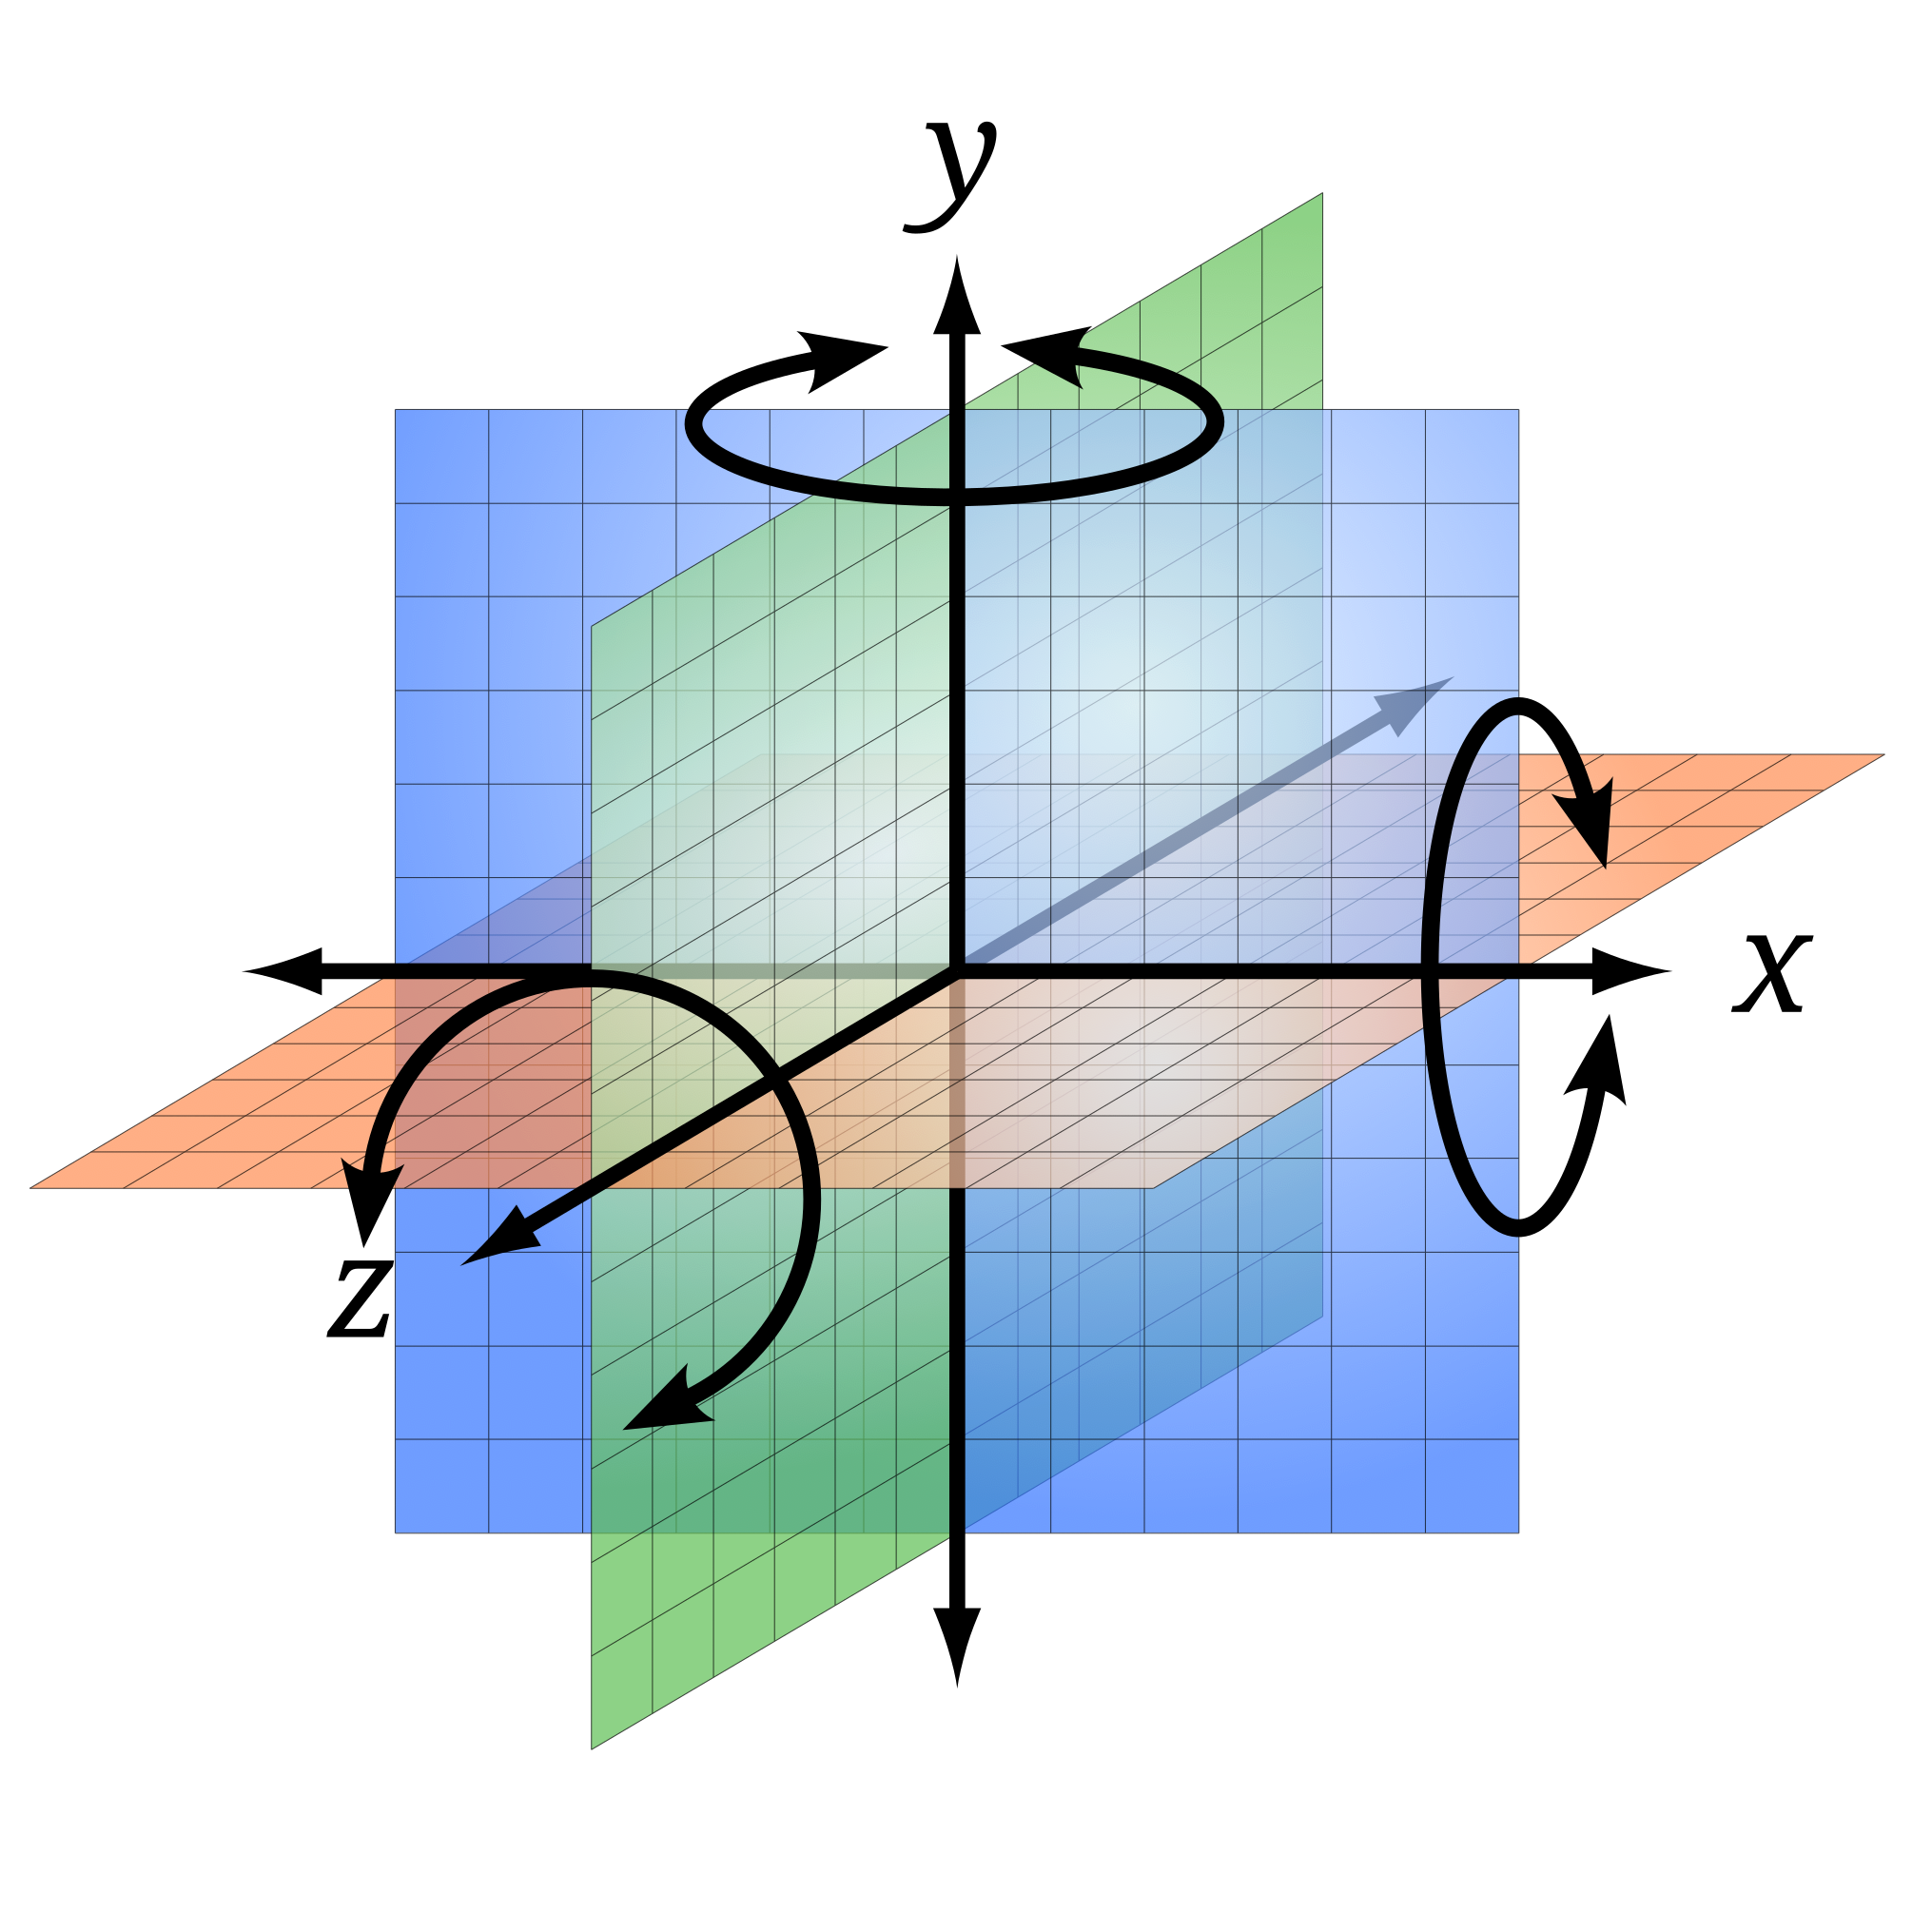
\includegraphics[width=5cm]{figs/coordinates.png}
  \end{center}
  \caption{Espacio tridimensional}
  \label{fig:espacio_tridimensional}
\end{figure}\ 

En base a lo anterior, con 3 grados de libertad no podremos situar el elemento terminal del manipulador en un punto del espacio 
y a la vez controlar la orientación de la herramienta en ese punto.\\

Seguidamente, se debe elegir el tipo de articulación que se pretende usar. En robótica, son ampliamente utilizados estos tipos de 
articulaciones:
\begin{itemize}
\item Revolución: Permite el movimiento de rotación alrededor de un eje fijo.
\item Prismático: Las partes del robot se pueden desplazar linealmente a lo largo de un eje específico. 
\item Esférico: Permite la rotación en cualquier dirección. Está restringido a 3 DOF y suele ser usado como articulación pasiva.
\item Cilíndrica: Permite el movimiento de rotación alrededor de un eje y también un desplazamiento lineal a lo largo del mismo. Combina los movimientos rotacionales y prismáticos. 

\begin{figure} [h!]
  \centering    
  \subfigure[Revolución 1 DOF]{\label{fig:j_rot}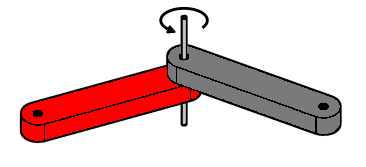
\includegraphics[width=0.3\linewidth ]{figs/joint_rot.png}}
  \hspace{1cm}
  \subfigure[Prismático 1 DOF]{\label{fig:j_prism}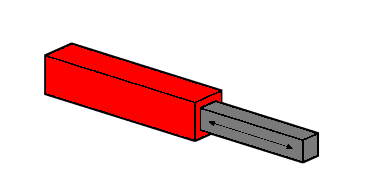
\includegraphics[width=0.3\linewidth]{figs/joint_prism.png}}
  \subfigure[Esférico 3 DOF]{\label{fig:j_esf}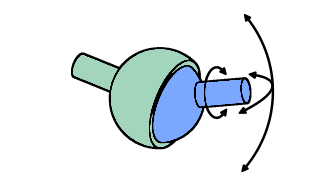
\includegraphics[width=0.3\linewidth ]{figs/joint_esf.png}}
  \hspace{1cm}
  \subfigure[Cilíndrico 2 DOF]{\label{fig:j_cil}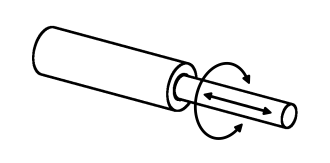
\includegraphics[width=0.3\linewidth]{figs/joint_cil.png}}
  \caption{Tipos de articulaciones más usadas en robótica}
\end{figure}

\end{itemize}

Se ha optado por articulaciones de tipo revolución, debido a que son sencillas de implementar y están compuestas por pocas partes 
móviles.

\newpage
Acto seguido, se debe establecer la forma del manipulador en función del tipo y número de articulaciones elegidas anteriormente. 
En base a las categorías de manipulador descritas en \ref{sec:rob_industrial}, se ha decidido implementar un robot basado 
en paralelogramos al estilo MeArm \ref{fig:mearm}.
\\ 
El tipo de brazo elegido tiene la peculiaridad de tener su elemento terminal siempre paralelo al suelo por lo que es ideal para 
tareas \textit{pick and place}. 

\section{Modelo alámbrico}
\subsection{En qué consiste}
\label{subsec:eqc_mod_alambrico}
El modelo alámbrico es una forma de analizar el movimiento de un sistema mecánico compuesto por ejes y eslabones. Este 
enfoque simplifica la representación visual al destacar las relaciones espaciales entre las diferentes partes del sistema mediante 
líneas y conexiones simbólicas, en lugar de mostrar detalles realistas del manipulador. 
\begin{figure} [ht!]
  \begin{center}
    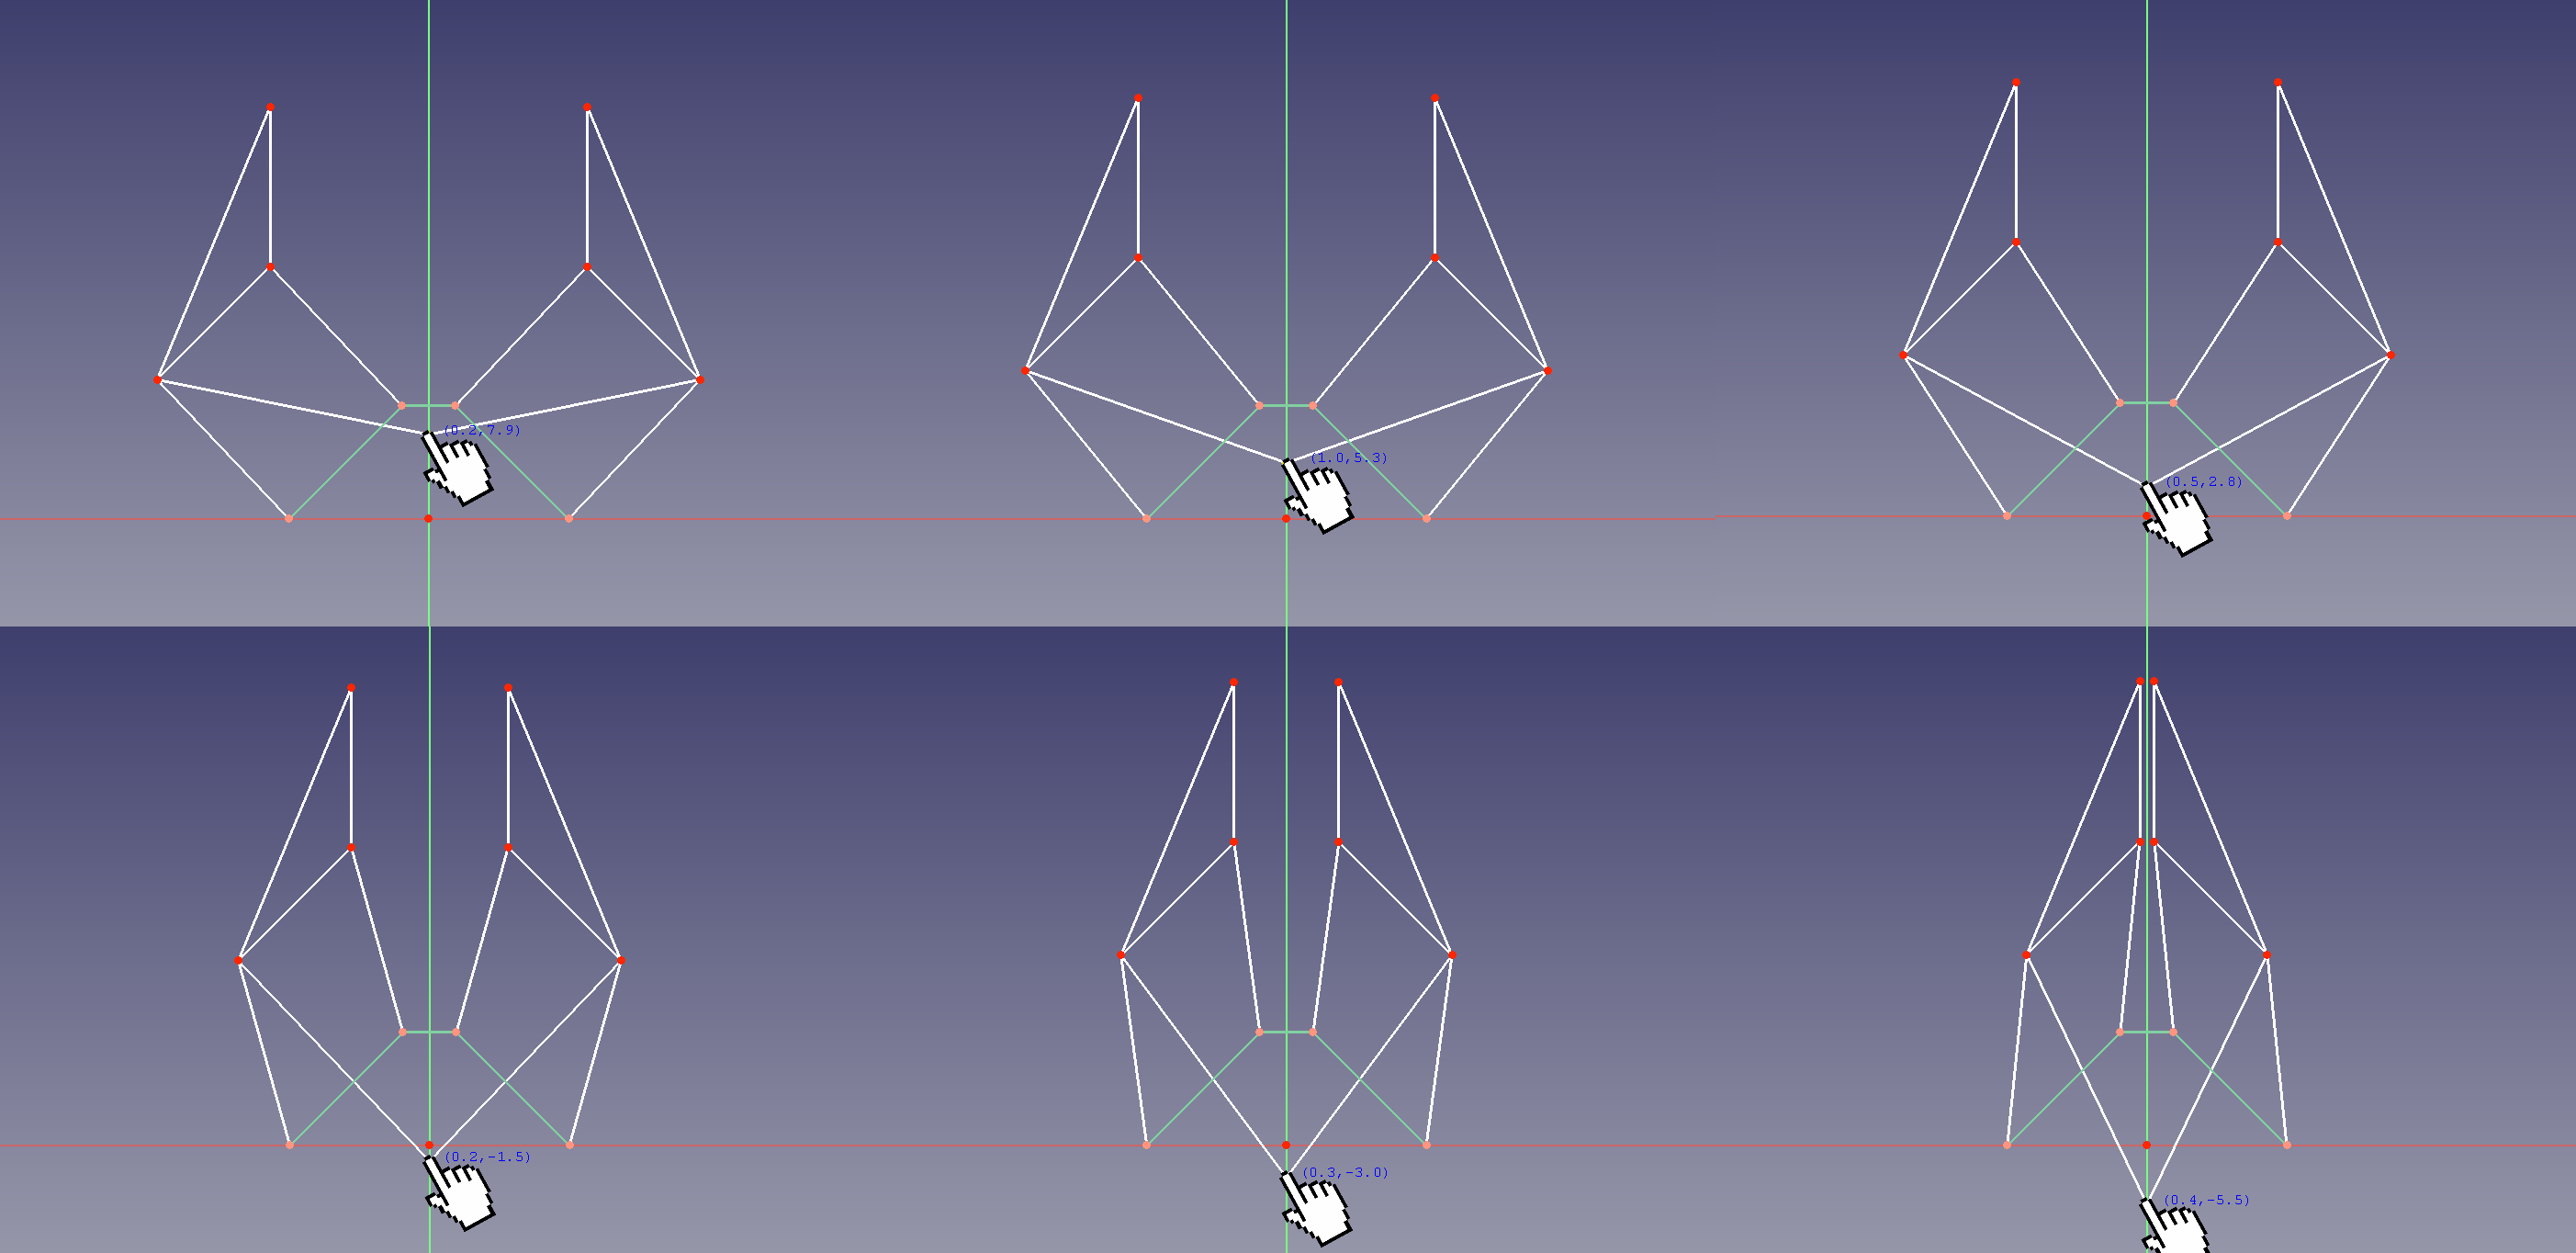
\includegraphics[width=15cm]{figs/pinza_evol.png}
  \end{center}
  \caption{Pinza paralela con 1 grado de libertad}
  \label{fig:mod_pinza_figure}
\end{figure}\ 

\newpage
\subsection{Desarrollo del modelo alámbrico de G-Arm}
\label{subsec:modelo_alambrico}
Para desarrollar el modelo alámbrico de este manipulador, se ha tomado como referencia el modelo alámbrico de MeArm del 
repositorio de github\footnote{\url{https://github.com/myTeachingURJC/Mecatronica/wiki/S3:-Estructuras-mec\%C3\%A1nicas-(II)}}. 
\\
Para abordar adecuadamente la modificación de modelo, es fundamental comprenderlo en su totalidad. Por suerte, el repositorio anterior  
contiene una explicación detallada de la razón de ser de cada elemento.

\begin{figure} [ht!]
  \begin{center}
    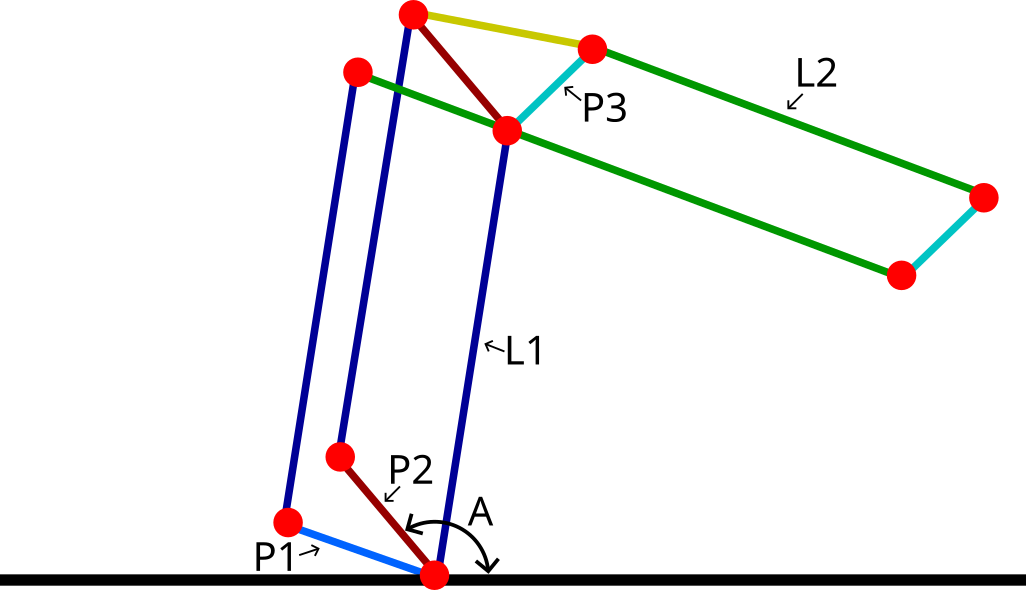
\includegraphics[width=15cm]{figs/mearm_params.png}
  \end{center}
  \caption{Parámetros del modelo alámbrico}
  \label{fig:mod_pinza_figure}
\end{figure}\ 

Este robot está definido por una serie de parámetros (L1, L2, P1, P2, P3, A). Para realizar la obtención de los parámetros que definen a 
G-Arm se ha utilizado la experimentación. El procedimiento ha consistido en modificar una medida y evaluar como se 
comporta a la hora de alcanzar ciertas zonas críticas. El objetivo final es encontrar una combinación de parámetros que 
permita alcanzar la mayor cantidad de puntos sin que sus eslabones intersecten entre sí. 

\newpage
Más concretamente, la obtención de los parámetros adecuados se realizó en el siguiente orden:
\begin{enumerate}
\item Una manera de comenzar, es estableciendo de antemano el largo de los eslabones primarios L1 y L2. En base al peso estimado de 
cada uno de ellos, y de los motores utilizados, ambos deberían medir 17cm o menos.
\item El siguiente paso es elegir P1, P2 y P3. Estos son los lados cortos del los paralelogramos. Es importante jugar con estos valores 
de tal manera que se consiga obtener los más largos posibles. Esto es debido a que las piezas reales ocupan un cierto espacio y si el paralelogramo es 
muy pequeño no realizarán todo el recorrido ya que chocarán entre sí. Codo
\item El ángulo A restringe el paralelogramo que mantiene el extremo del robot paralelo al suelo.   
\end{enumerate}
En esta imagen se muestra el modelo alámbrico de G-Arm:\\
\begin{figure} [ht!]
  \begin{center}
    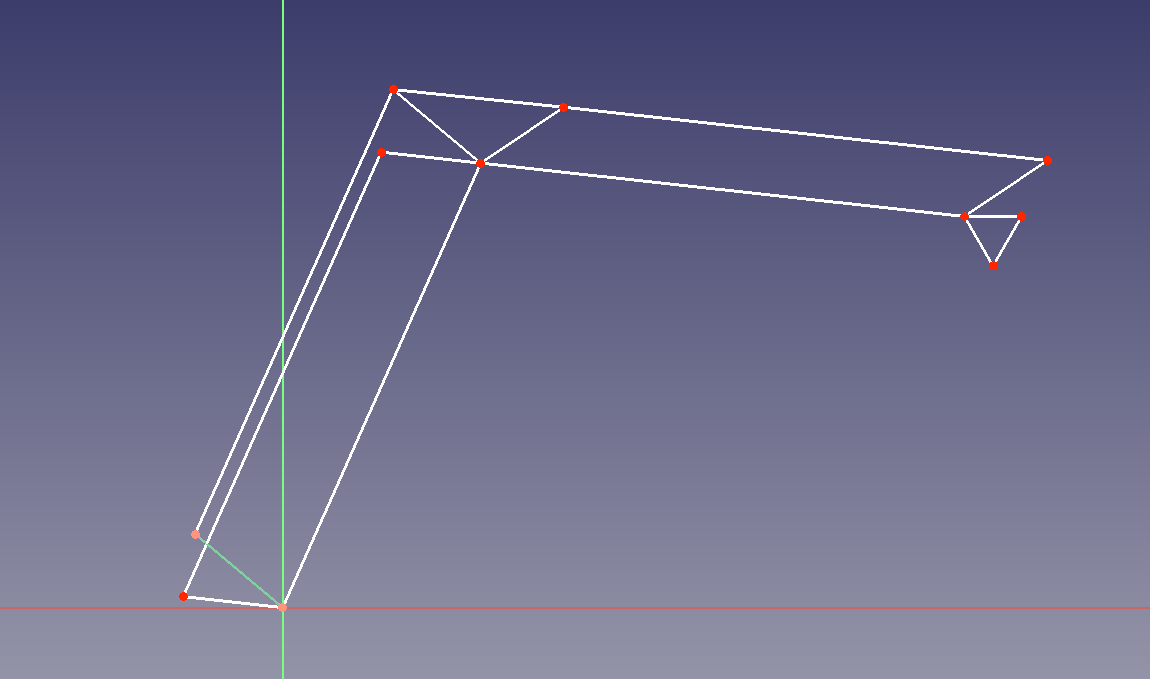
\includegraphics[width=15cm]{figs/alambrico_garm.png}
  \end{center}
  \caption{Modelo alámbrico de G-Arm}
  \label{fig:mod_pinza_figure}
\end{figure}\ 
Revisar parametros
\newpage
En la siguiente tabla se muestran los valores obtenidos: 
\begin{table}[H]
\begin{center}
\begin{tabular}{|c|c|}
\hline
\textbf{Parámetros} & \textbf{Valores} \\
\hline
L1 & 170mm \\
L2 & 170mm \\
P1 & 35mm \\
P2 & 35mm \\
P3 & 25mm \\
A & 135º \\
\hline
\end{tabular}
\caption{Parámetros del modelo alámbrico de G-Arm}
\label{cuadro:parametros_alambrico}
\end{center}
\end{table}

\section{Bocetos}
Una parte importante del diseño son los bocetos previos al modelado 3D. En estos bocetos se busca tener una idea clara de la forma 
y posición de cada pieza, así como de su lugar en el espacio.  
Para el desarrollo de este brazo, se han realizado numerosos bocetos, de los cuales se conservan aquellos dibujados digitalmente en 
un iPad.
\section{Elección de componentes hardware}
En esta sección se analiza las necesidades que deben satisfacer los componentes hardware (motores, placas, fuentes de alimentación etc.)
y se busca la mejor opción rendimiento-precio existente en el mercado. 

\subsection{Motores}
Según la geometría establecida en \ref{sec:eligiendo_geometría}, el robot necesita 3 motores. Los utilizados en este proyecto deben
cumplir las siguientes características:
\begin{enumerate}
  \item Deben ser capaces de entregar el suficiente torque para levantar el brazo más una cierta la carga en su extremo.
  \item Se debe poder conocer su posición en cada instante.
  \item Deben poder mantener su torque sin estar en movimiento.
\end{enumerate}

Debido a esta última necesidad, no es buena idea usar motores convencionales de corriente contínua con escobillas, ya que no son 
capaces de aportar torque sin girar. Por otro lado, los motores paso a paso si son capaces de ello y, aunque no estén codificados,
se puede conocer la posición relativa ya que avanza en pequeños incrementos discretos (pasos). Además, este tipo de motor es capaz de 
entregar un torque considerable para su tamaño. Por contra, son bastante pesados. 

Tras investigar las opciones existentes en el mercado, se ha llegado a la conclusión que los motores Nema 17 son la opción ideal 
para la realización de este trabajo debido a que son comunes y fáciles de encontrar, además de tener un precio aceptable. Aún así, 
existen motores Nema de diferentes tamaños, para realizar robots más o menos grandes.
\begin{figure} [ht!]
  \begin{center}
    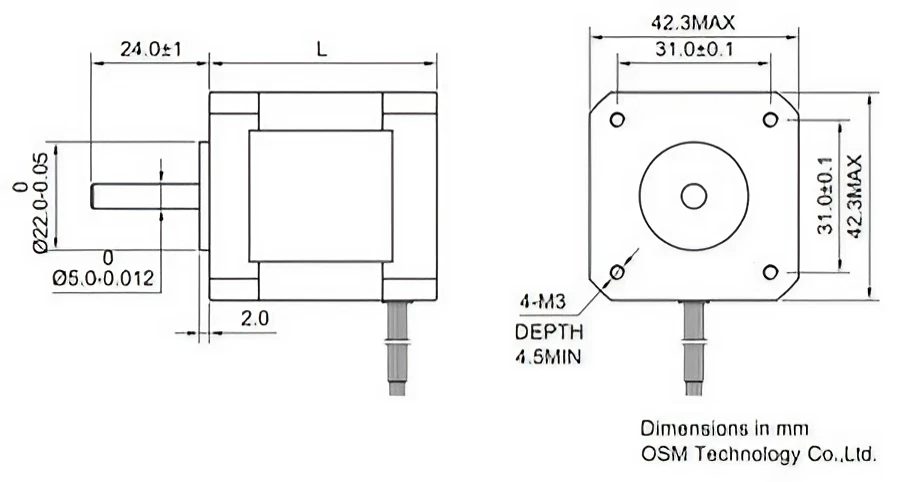
\includegraphics[width=15cm]{figs/MotorsNema.png}
  \end{center}
  \caption{Diferentes categorías de motor paso a paso Nema \footnote{\url{https://filament2print.com/es/blog/139_motores-nema.html}}}
  \label{fig:nema}
\end{figure}\ 

Dentro de la categoría Nema 17, todos tienen el mismo factor de forma a excepción del largo del motor. Esta característica determina 
el torque del motor. A mayor longitud, mayor torque es capaz de ejercer. 

Fotito de lo necesario

\subsection{Reductora}
Para poder reducir la velocidad de giro de un motor y, a su vez convertirla en fuerza, es necesario implementar una reductora. 
Existen diferentes formas de hacerlo, como pueden ser los engranajes (normales, planetarios, helicoidales...) y las correas (lisas y 
dentadas).

Se ha optado por el uso de correas dentadas sobre el uso de engranajes, debido a que estos últimos siempre añaden una cierta holgura 
al movimiento final, haciendo el robot inexacto y añadiendo incertidumbre en los movimientos. Las correas dentadas en cambio, utilizan 
tensores para asegurar que siempre está en contacto con ambas poleas.

Foto de correa dentadas
Se pretende usar correas de tipo GT2. Este tipo de correa es ampliamente utilizado en impresoras 3D, por lo que es realmente económico y 
fácil de encontrar. Dentro de esta categoría existen diferentes anchos de correa en función de la tensión soportada. En este caso, 
se ha elegido el ancho de 6mm puesto que es el más económico con diferencia y es más que suficiente para esta aplicación.En la construcción 
de robot industriales caseros y profesionales de metal y de gran tamaño, se utilizan correas y cadenas con mayor grosor y tamaño de diente.
Foto de mi correa.

Además, las poleas necesarias para este tipo de correas son fáciles de diseñar e imprimir en 3D, lo que permite hacer poleas con 
un número de dientes concreto y por un precio casi nulo.

En este caso, para dos de los grados de libertad, se ha elegido utilizar una polea comercial de 20 dientes de metal unida al 
eje del motor en conjunto con otra de 100 dientes impresa en 3D, logrando así una reducción de 1:5. En el grado de libertad restante, 
se pretende utilizar el mismo concepto pero con una polea de 120 dientes (Reducción 1:6).

\subsection{Controladores}
Debido a que se prentende utilizar motores paso a paso bipolares, es necesario utilizar un tipo de electrónica específica para 
este tipo de motor. Este componente hardware es llamado controlador, y su objetivo es convertir una señal eléctrica del controlador 
en una serie de pulsos de mayor potencia que excitarán las bobinas del motor. 
Para motores paso a paso de baja corriente (hasta 2A), existe un formato de forma común en el mundo \textit{maker}. Es por esto que la 
mayor parte de los controladores paso a paso que encontramos en el mercado son intercambiables entre sí. La diferencia entre ellos, reside 
en la tecnología de su interior y las capacidades técnicas que ofrecen. 
\begin{table}[htbp]
  \centering
  \caption{Comparación de especificaciones de los controladores existentes}
  \begin{tabular}{|c|c|c|c|c|c|}
      \hline
      \multirow{2}{*}{Modelo} & Voltaje de & Corriente & \multirow{2}{*}{Microstepping} & Nivel de & \multirow{2}{*}{Precio} \\
                             & alimentación & máxima & & ruido &\\
      \hline
      A4988 & 8-35V & 2A & Hasta 1/16 & Muy ruidoso & 1\euro \\
      \hline
      DRV8825 & 8.2-45V & 2.5A & Hasta 1/32 & Ruido aceptable & 2\euro \\
      \hline
      TMC2225 & 4.7-36V & 2A & Hasta 1/32 & Bajo ruido  & 2.8\euro \\
      \hline
      TMC2208 & 4-35V & 2A &  Hasta 1/256 & Totalmente silencioso & 2.8\euro \\
      \hline
      TMC2209 & 5.5-28V & 2.5A & Hasta 1/256 & Totalmente silencioso & 3.4\euro \\
      \hline
  \end{tabular}
\end{table}

Debido a que se pretende utilizar motores Nema 17 de más de 2A, la decisión debe estar entre el DRV8825 y el TMC2209. Finalmente, se 
ha elegido este último debido a que es realmente silencioso e incorpora una tecnología superior que garantiza una señal más definida que 
evita la pérdida de pasos del motor. Además, a la hora de adquirirlo, suele venir acompañado de un disipador de calor más grande que, unido 
a su mayor eficiencia energética, se traduce en una menor cantidad de calor dentro de nuestro robot. 

\subsection{Placa base}
La placa base es una targeta de circuito impreso que proporciona conexiones físicas y eléctricas entre las diferentes componentes y 
unifica estos en un mismo componente. 
En el caso de aquellas usadas para montar controladores paso a paso, suelen integrar un \ac{MCU} o actuar como un \textit{shield} 
(placa adicional que se acopla a otras para aumentar su funcionalidad y características).
Foto cnc arduino shield y otras

Existen numerosas opciones en el mercado con la posibilidad de montar una distinta cantidad de controladores. En el caso de este 
trabajo necesitamos sólamente 3. Este tipo de placas suelen ser utilizadas para crear máquinas CNC y en este caso se ha optado por 
elegir una placa económica que integra todo lo necesario para este proyecto a exccepción de los controladores. 
Se ha elegido esta y no otra puesto que tiene un \acs{MCU} ESP32 muy superior al AtMega328p del Arduino Uno. Además cuenta con la 
capacidad de poderse controlar vía wifi y la mayor ventaja es que incorpora un mosfet conectado a una salida pwm a la que podemos conectar 
un motor de hasta x vatios, un electroimán etc. Además incluye una serie de pines y salidas muy cónmodas de utilizar para montar 
módulos de grabado láser y etc. Todo ello por un precio de 16€.

\subsection{Fuente de alimentación}
Se trata de un elemento clave del robot. Es importante conocer \textit{a priori} las 
características necesarias de la fuente.

Por ello, se ha realizado una estimación del consumo del robot final. La mayor parte del consumo viene dado por los propios motores que 
se encontrarán permanentemente excitados con el fin de mantener el robot en una determinada posición sin desplomarse. Según las especificaciones 
de los motores escogidos, cada uno consume en torno a 7W. Es decir, el consumo de los motores es de 21W. A esto hay que añadir el consumo del 
microcontrolador y de los controladores (unos 4W). Además, si se quiere añadir un electroimán al extremo o algún servo, se necesitará de 
un extra de potencia. 
En base  a la estimación, se establece que lo ideal y recomendable para alimentar este equipo es una fuente de alimentación de 12 a 24V capaz 
de entregar al menos 30W. Si se desea usar una fuente de baja calidad, lo ideal es elegir una un 30\% más potente para evitar forzarla y aumentar 
su vida útil.
Debido al amplio rango de voltaje y de su bajo consumo, es perfectamente alimentable con un cargador típico de portátil de 19V sin temor 
a dañarlo. Pese a esto, se ha decidido utilizar una fuente de alimentacion genérica de 24V 150W para poder realizar \textit{a posteriori} 
todas las mediciones de consumos descartando a la fuente como factor limitante. El precio de esta fuente es de 15\euro.
\newpage
\subsection{Rodamientos}
Para mejorar la eficiencia de las articulaciones y garantizar que todas roten con suavidad, se pretende hacer uso de rodamientos 
en cada una de ellas. 
Existen diferentes tipos de rodamientos en el mercado pero se ha elegido un tipo de rodamiento específico para este propósito. 
Se ha optado por el uso de rodamientos brida como el de la Figura \ref{fig:rodamientos_fushi}. Este tipo de rodamientos son usados en las poleas pasivas de las impresoras 3D, por lo 
que son muy baratos (10 de buena marca por 6-10€) y sencillos de encontrar. La razón principal de su uso es su peculiar forma. Este tipo 
de rodamiento tiene un borde en el extremo que hace de borde. Esto lo hace ideal para insertar en las piezas 3D a desarrollar y garantizar 
que nunca se puedan sacar mientras el tornillo este fijado. Además evita que el rodamiento se mueva y se gire cuando la articulación 
recibe un esfuerzo lateral. (Véase la Figura \ref{fig:ejemplo_rodamiento})

\begin{figure} [ht!]
  \centering  
  \subfigure[Rodamientos F695-2RS Fushi \footnote{\url{https://es.aliexpress.com/item/32850989216.html}}]{\label{fig:rodamientos_fushi}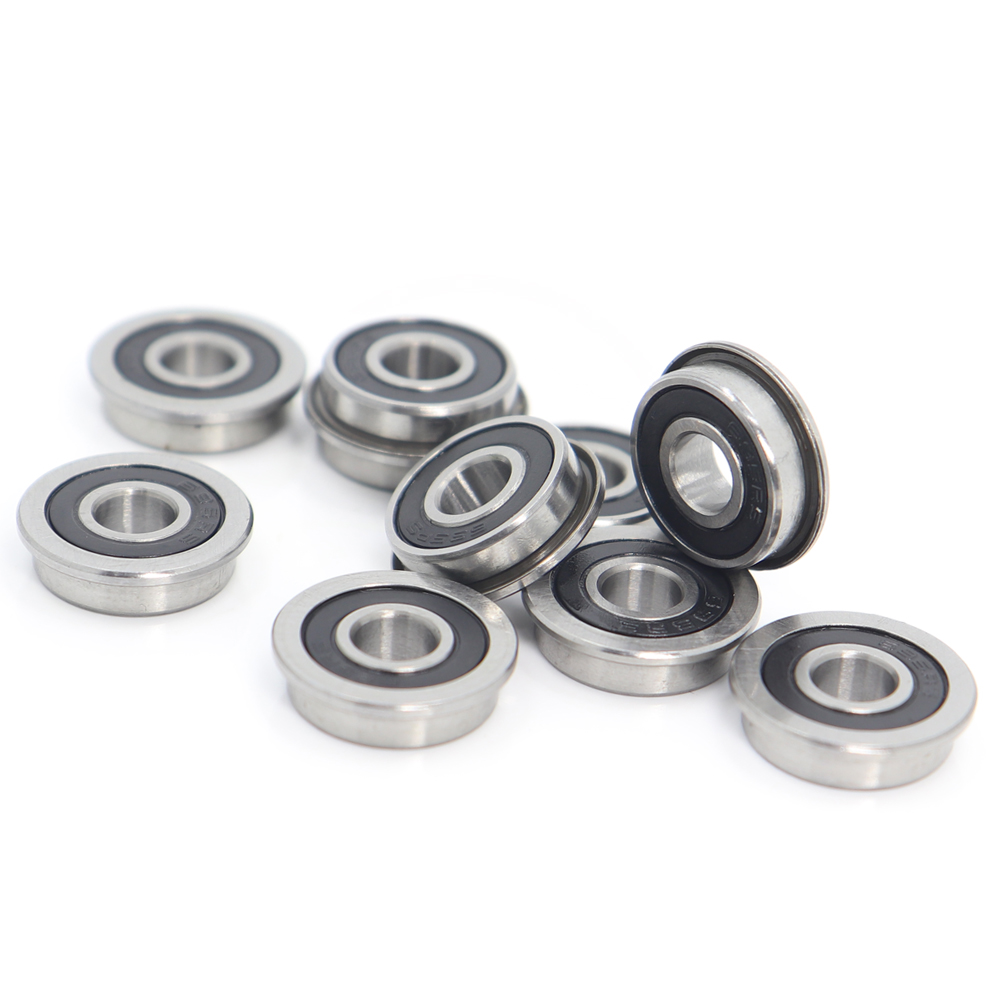
\includegraphics[width=0.4\linewidth ]{figs/F695-2RS.jpeg}}
  \hspace{0.5cm}
  \subfigure[Ejemplo de uso]{\label{fig:ejemplo_rodamiento}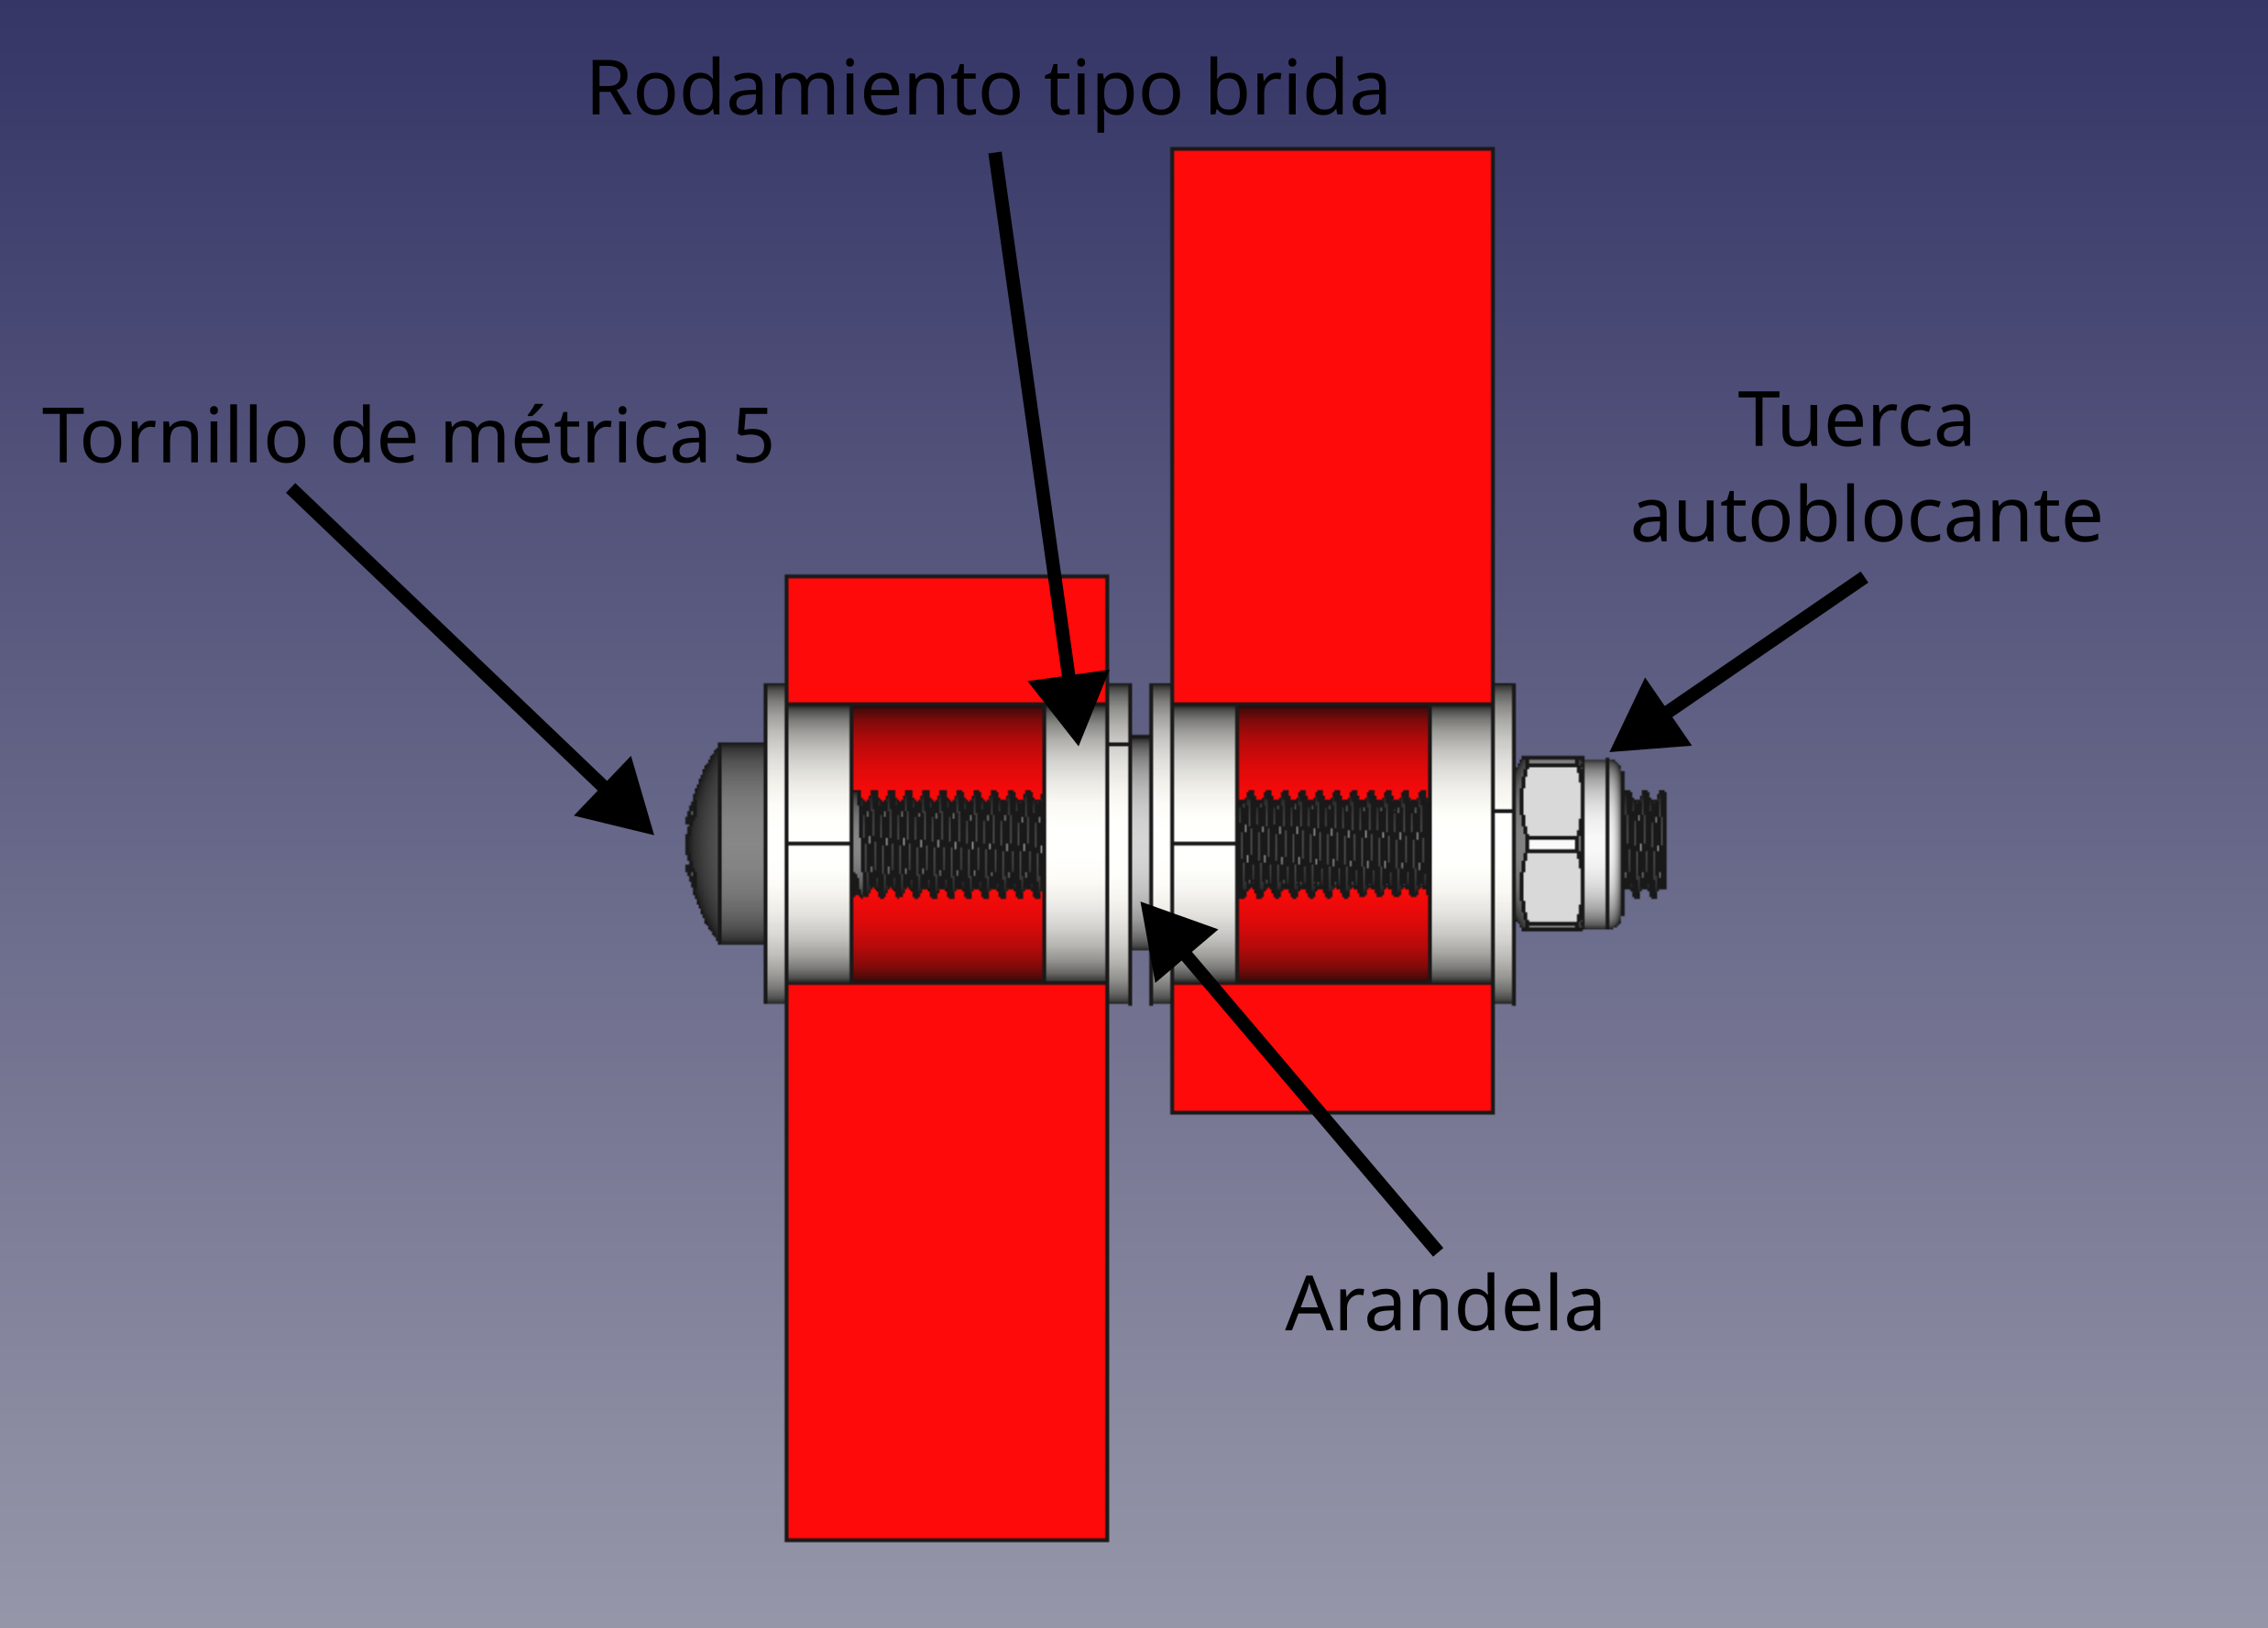
\includegraphics[width=0.5\linewidth ]{figs/RodamientosBrida.png}}
  \caption{Rodamientos de tipo brida}
\end{figure}\ 

\subsection{Finales de carrera}
Son útiles para conocer el final del recorrido de una articulación y poder establecer la posición absoluta al inicio de la 
máquina. 
Existen cantidad de ellos en el mercado y con distintas tecnologías. Se ha decidido utilizar unos basados en \textit{microswitches} debido a 
que son baratos y cumplen su función. Además son compatibles con la placa previamente elegida. 
\subsection{Electroimán}
Para realizar las pruebas, se pretende crear una herramienta para el robot que consiste en un electroimán para poder mover objetos metálicos 
de sitio. En el mercado existen muchos tipos de electroimán con distintos consumos y fuerzas. Uno ideal para esta aplicación es el \textit{D20H15}.
Su nombre indica que es un electroimán de diámetro 20mm y altura 15mm. Según las especificaciones del producto, es capaz de levantar hasta 3Kg. 
Además, es necesario comprar la versión de 24v para poder alimentarlo con tensiones entre 18 y 24v. En caso de alimentar el robot con 12v, se debería 
adquirir la versión de 12 para poder aprovechar toda su fuerza. El consumo de este electroimán es de 3W.
\newpage
\section{Diseño CAD}
En esta sección se va a hablar de las particularidades del diseño y diversos aspectos a tener en cuenta a la hora de diseñar 
cualquier pieza mecánica que posteriormente será impresa en 3D. 
\\
Para el diseño de este brazo robot, se ha utilizado dos herramientas de diseño. Inicialmente el proyecto se realizó mediante 
la herramienta \textit{Fusion 360} y posteriormente se utilizó FreeCad\ref{sec:freecad} para cumplir con el objetivo de ser totalmente 
\textit{Open Source} y estar parametrizado, para que cualquier persona pueda investigarlo, modificarlo y utilizarlo de forma gratuita.
\\ 

\subsection{Base principal}
Este conjunto es el encargado de unir el resto del robot al suelo. Dentro de ella debe encontrarse la placa base junto con los controladores 
y toda la electrónica a excepción de la fuente de alimentación. Esto es así debido a que se puede alimentar de múltiples formas (baterías, 
cargadores de ordenador, fuentes de PC, salidas de alimentación de robots móviles, etc). Además, esta electrónica debe poder estar refrigerada 
por un pequeño ventilador incorporado en la propia base. \\
Se optó por realizar dos piezas circulares y una serie de espaciadores anchos que unían el conjunto, dejando espacio en el interior para 
la placa base. Este tipo de piezas son muy robustas y fáciles de imprimir. 
\begin{figure} [ht!]
  \begin{center}
    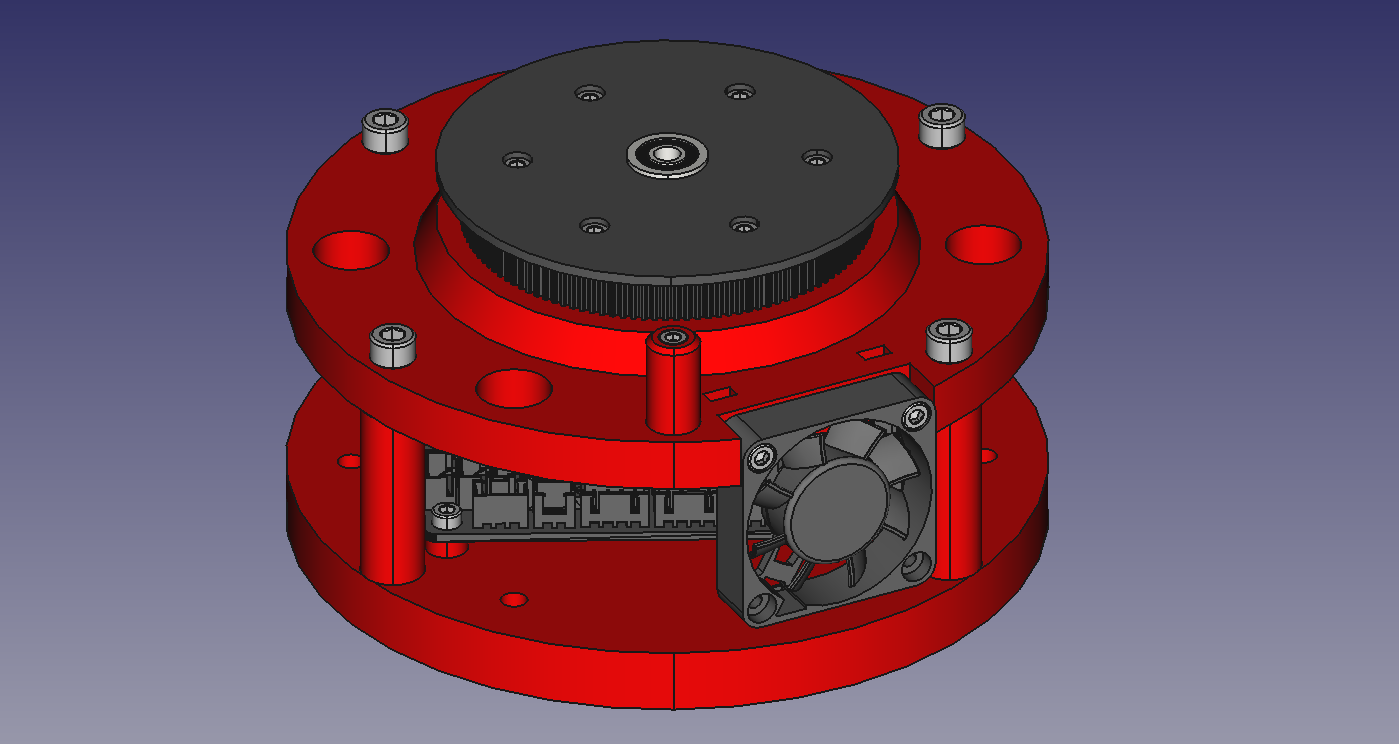
\includegraphics[width=12cm]{figs/base_principal.png}
  \end{center}
  \caption{Base principal}
\end{figure}\ 

\subsubsection{Pieza circular superior}
La pieza circular superior (Figura \ref{fig:base_principal_superior}), incluye una serie de agujeros y huecos hexgonales para insertar las tuercas M3 que permiten
acoplar la polea de 120 dientes (Figura \ref{fig:base_principal_polea}). Además, incluye un rebaje de 40mm en un lateral para poder insertar y atornillar un ventilador 4010.
\subsubsection{Espaciadores}
Los espaciadores (Figura \ref{fig:base_principal_espaciadores}) constan de 4 cilindros perforados con un agujero de 5mm por el que entrarán los tornillos de métrica 5.
\subsubsection{Pieza circular inferior}
La pieza circular inferior (Figura \ref{fig:base_principal_inferior}), contiene una serie de agujeros para poder atornillar la placa base. Además contiene una serie de agujeros en su perímetro 
para poder atornillar el robot al suelo. 

\begin{figure} [ht!]
  \centering    
  \subfigure[Polea 120 dientes]{\label{fig:base_principal_polea}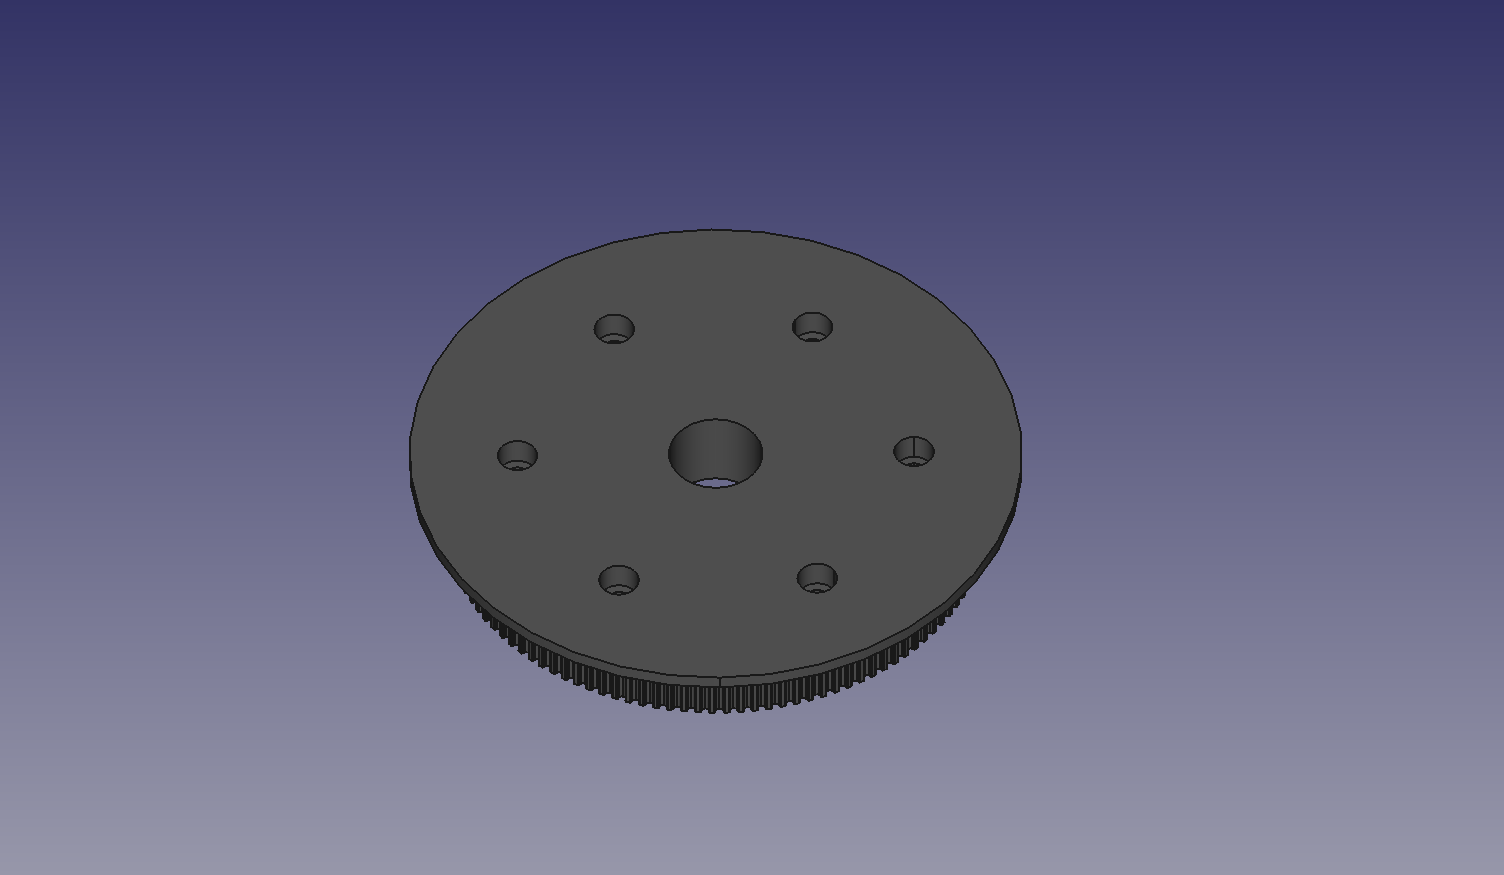
\includegraphics[width=0.45\linewidth ]{figs/base_principal_polea.png}}
  \hspace{1cm}
  \subfigure[Pieza superior]{\label{fig:base_principal_superior}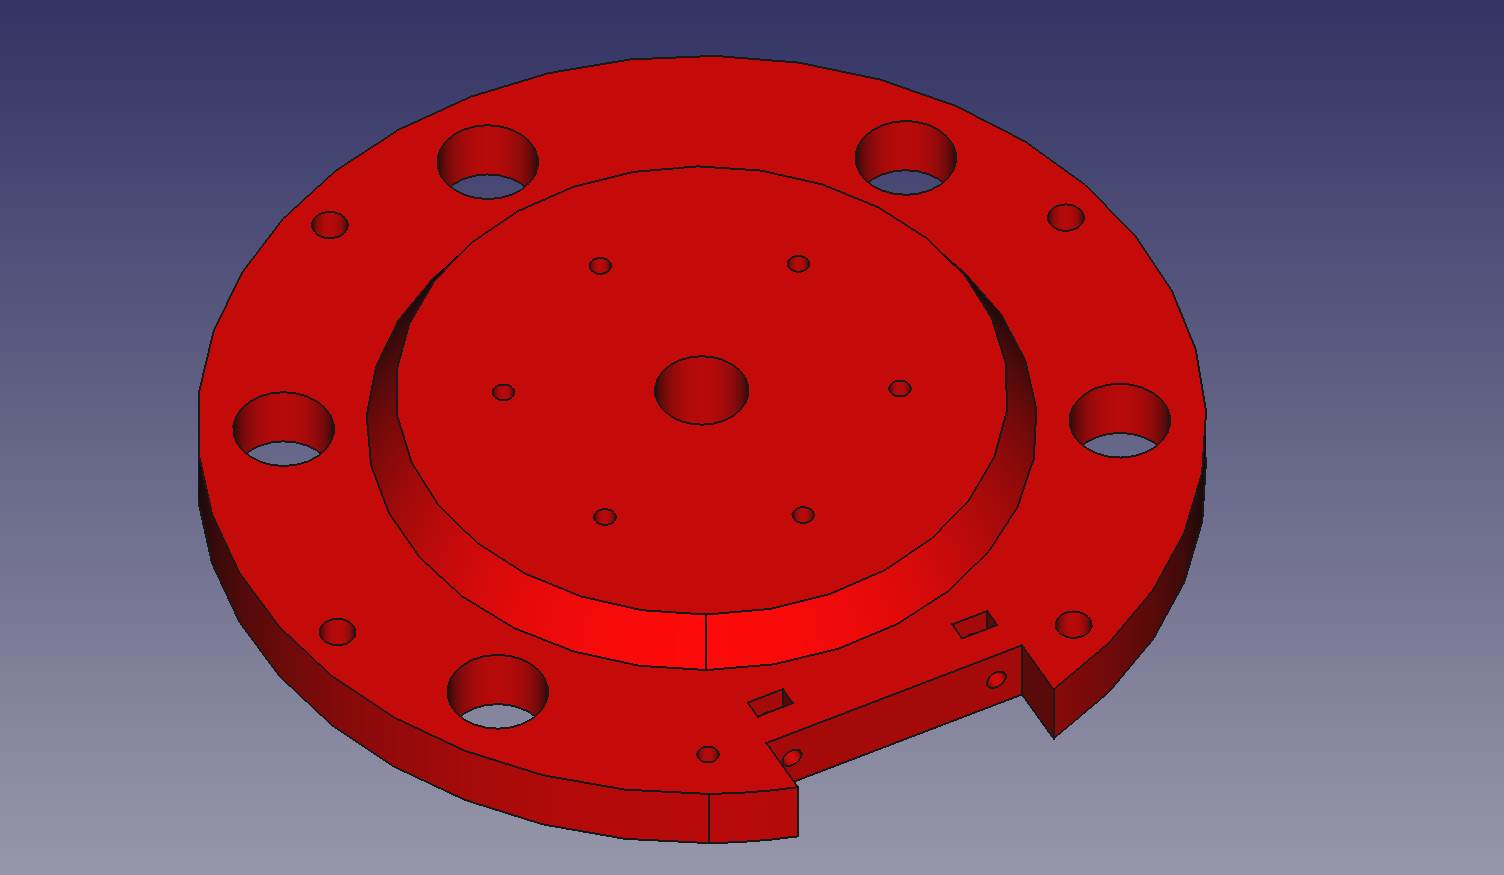
\includegraphics[width=0.45\linewidth]{figs/base_principal_superior.png}}

  \subfigure[Espaciadores]{\label{fig:base_principal_espaciadores}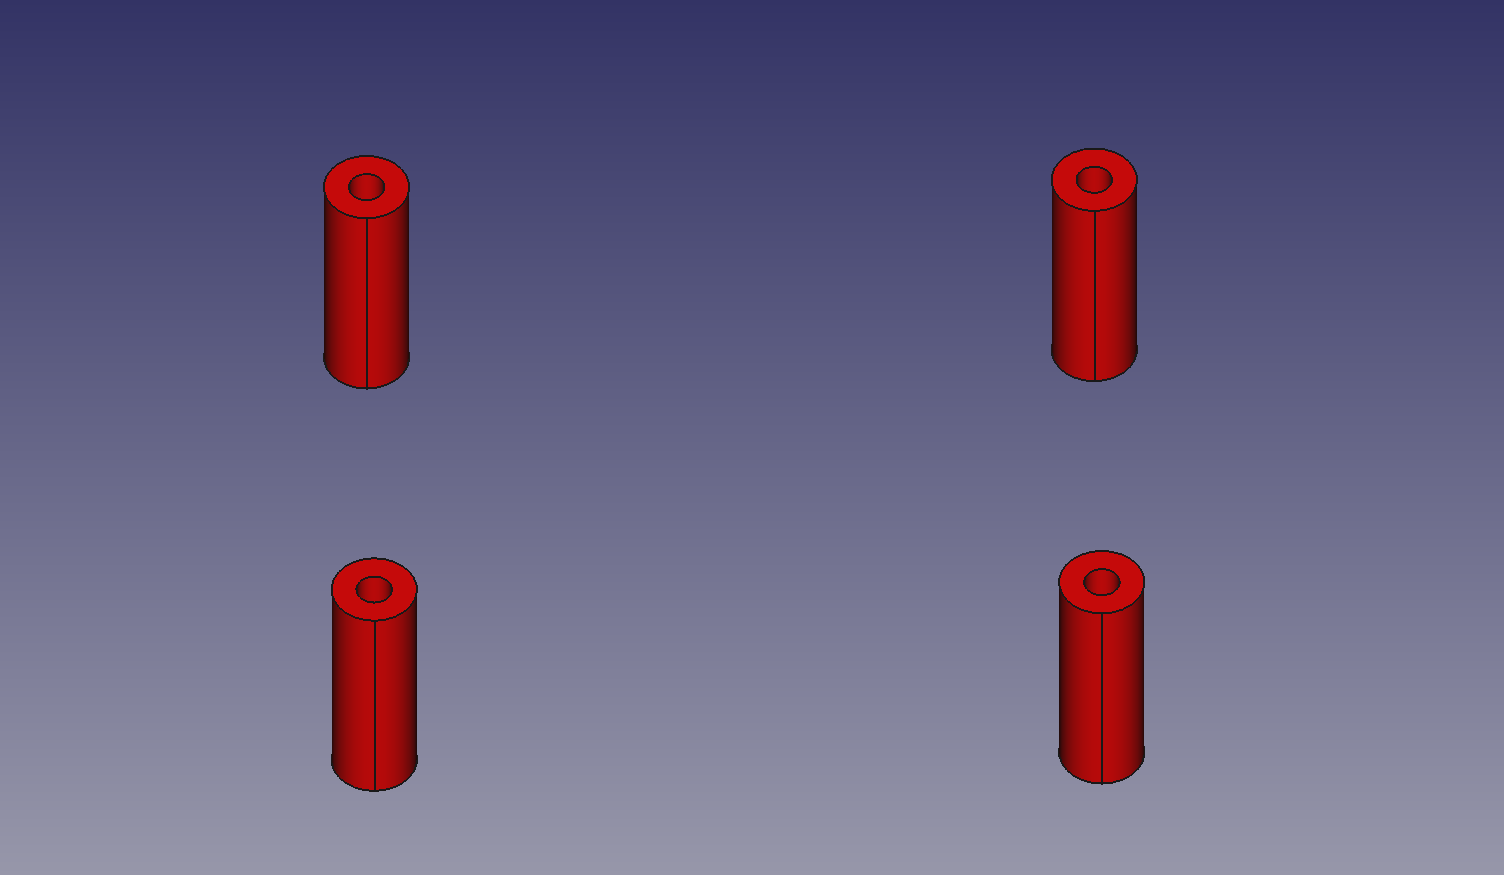
\includegraphics[width=0.45\linewidth]{figs/base_principal_espaciadores.png}}
  \hspace{1cm}
  \subfigure[Pieza inferior]{\label{fig:base_principal_inferior}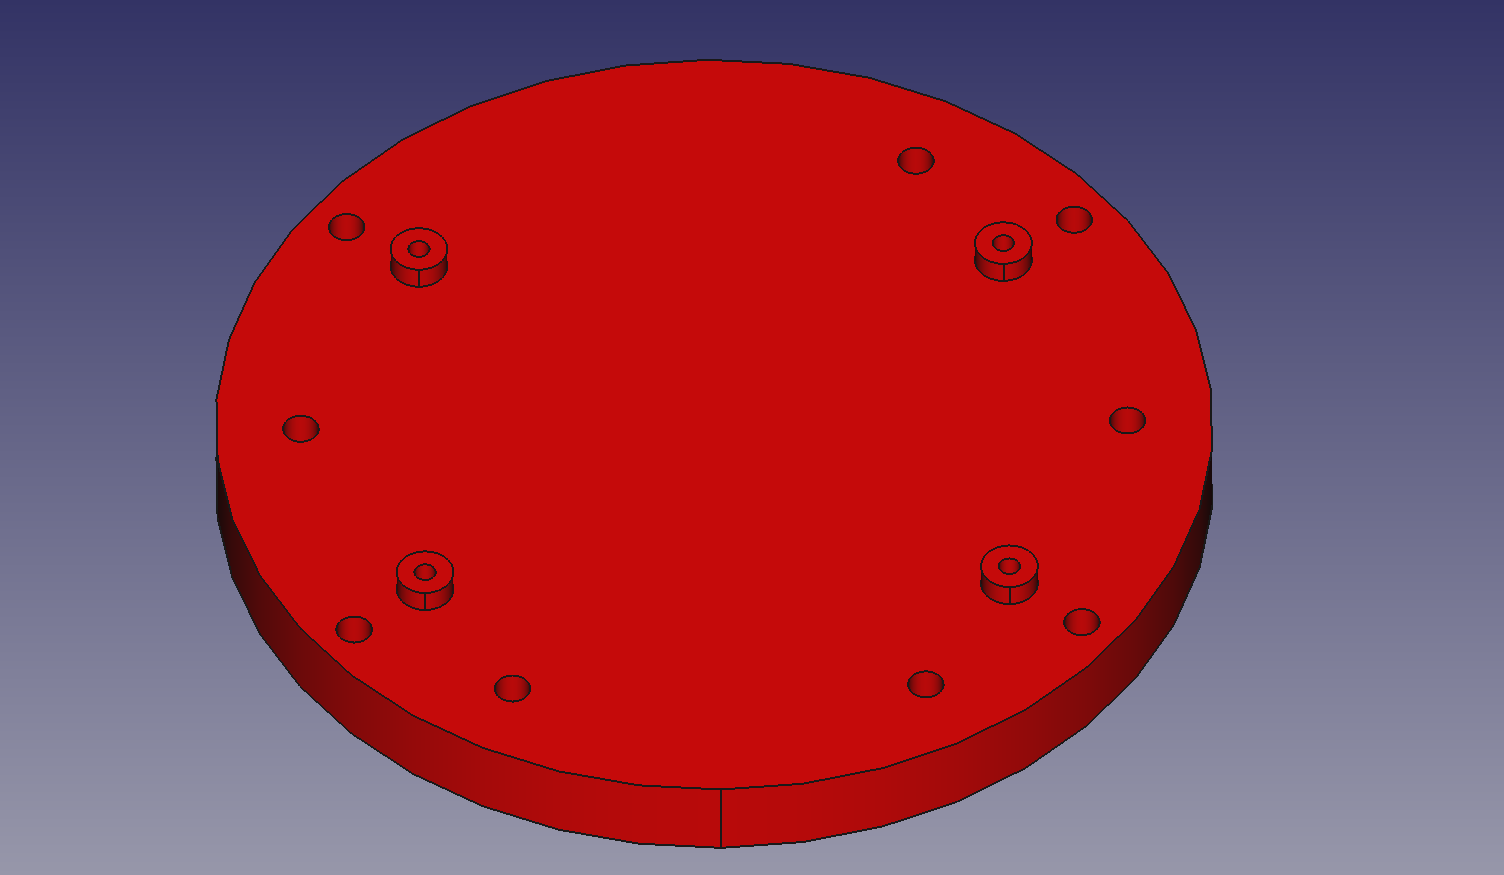
\includegraphics[width=0.45\linewidth]{figs/base_principal_inferior.png}}
\end{figure}
\newpage
\subsection{Base de los motores}
\noindent Este conjunto es el encargado de contener los 3 motores y rotar sobre la base principal
\begin{figure} [ht!]
  \begin{center}
    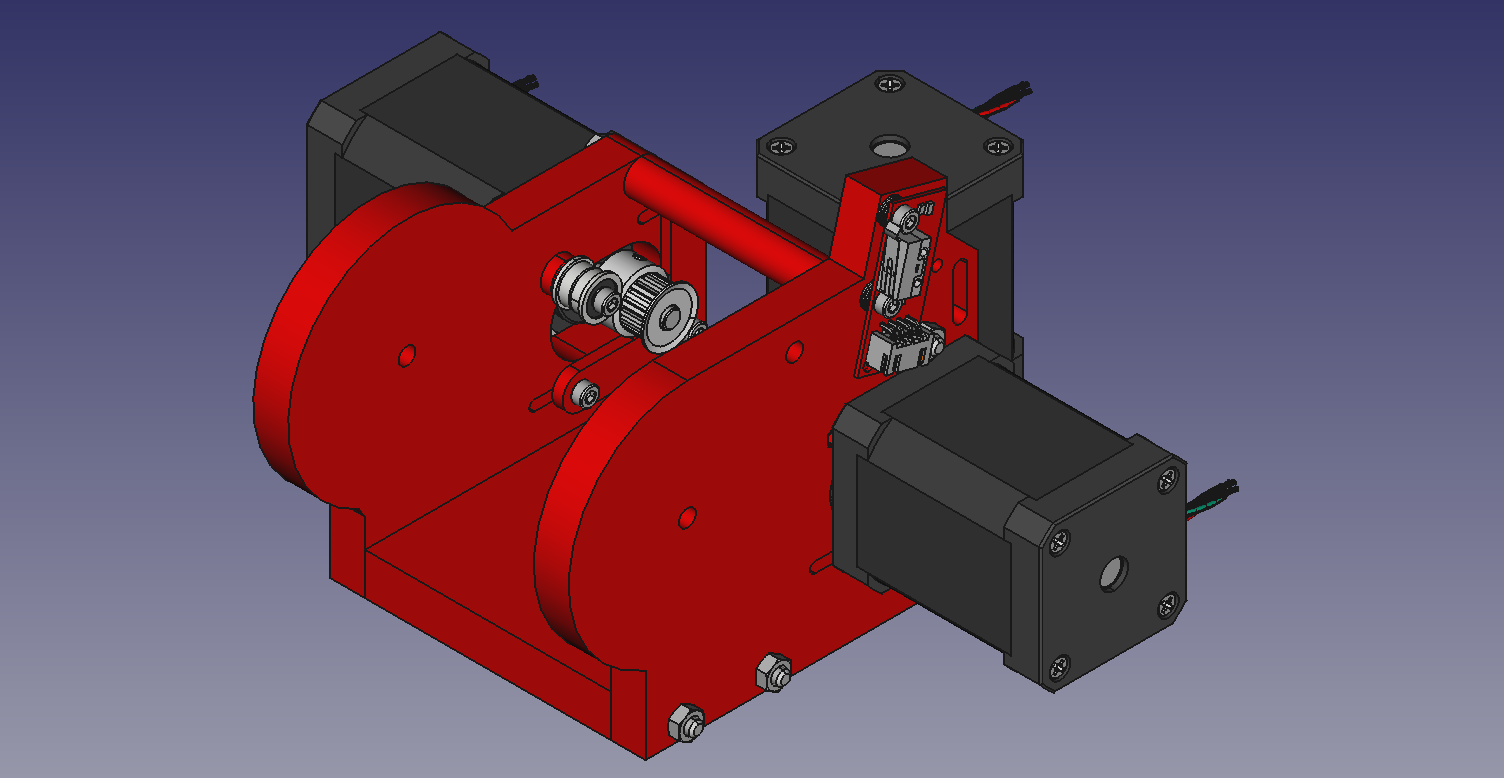
\includegraphics[width=12cm]{figs/base_motores.png}
  \end{center}
  \caption{Base de los motores}
\end{figure}\ 
\\
Consiste principalmente en 4 piezas; las dos laterales, la inferior y un espaciador de lado a lado que refuerza el conjunto. Esta ideado así 
para realizar piezas que serán imprimidas en dirección horizontal que es como mayor resistencia tienen las piezas en impresora 3d por la 
dirección de las capas. Además se consigue la máxima exactitud en los orificios y formas circulares. Todo el conjunto se une a través de 
varillas roscadas y tuercas.

Cabe recalcar el sistema de tensado de las correas. Consiste en una serie de orificios longitulidanes y una pieza que agarra el motor por 
el otro lado a modo de sandwich.
foto de lateral que se vea eso

Además esta pieza incorpora 2 de los 3 finales de carrera del robot. Además tiene una serie de ranueras para poder poner bridas a posteriori y 
organizar bien los cables.
\subsection{Paralelogramos}
\newpage
\subsection{Elemento terminal}
\noindent Esta pieza (Figura \ref{fig:extremo_pieza}) está la situada en el extremo del robot. Es la encargada de realizar la unión entre el robot y la herramienta. Por esto, 
se ha ideado con una forma particular que permite acoplar herramientas de una forma sólida e inequívoca. 
\begin{figure} [ht!]
  \begin{center}
    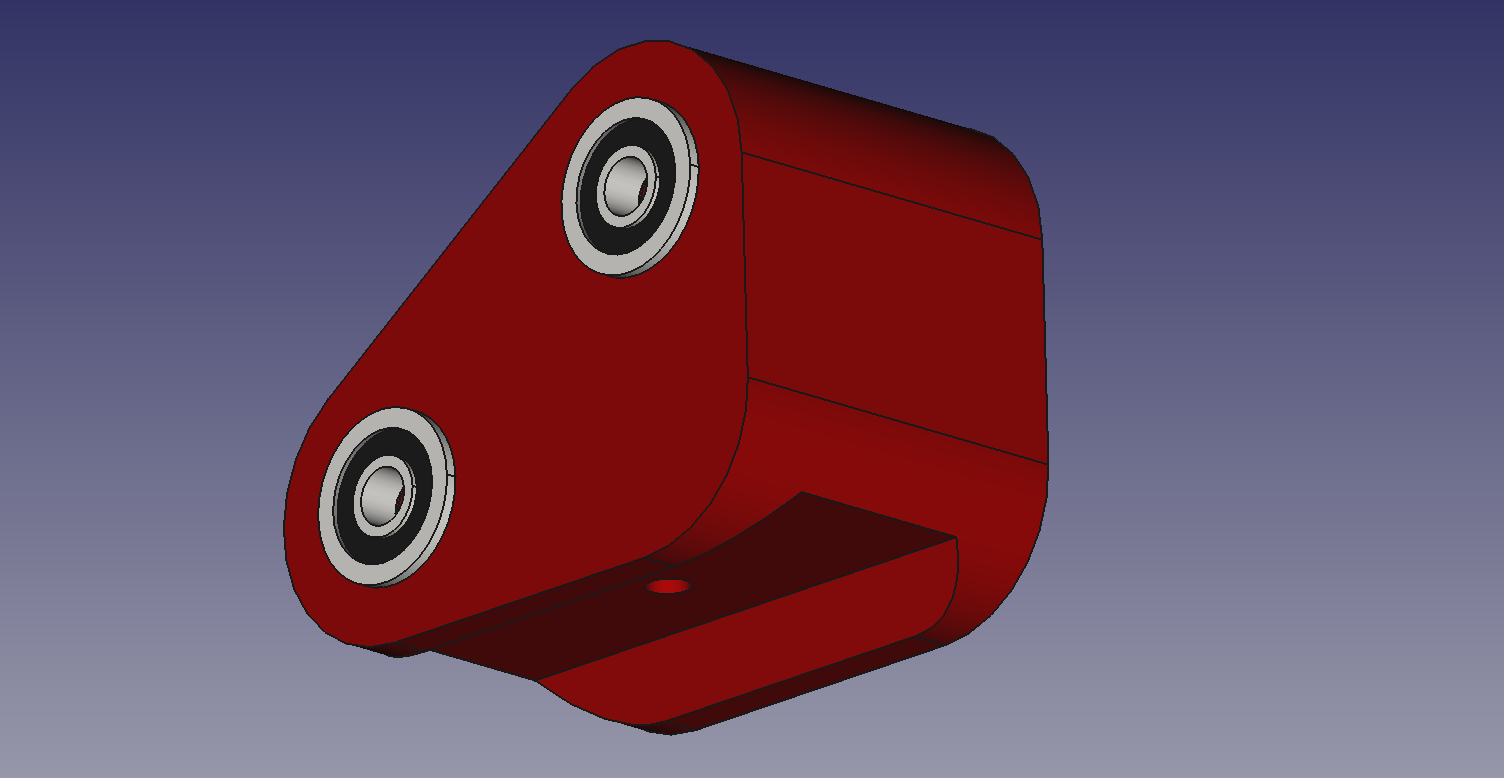
\includegraphics[width=10cm]{figs/extremo_robot.png}
  \end{center}
  \caption{Elemento terminal}
  \label{fig:extremo_pieza}
\end{figure}\ 
\\
Consiste en una acanaladura a 45 grados (Figura \ref{fig:vistas_extremo}) con un agujero que la atraviesa, por el que pasará el tornillo unirá ambas piezas. 
Este acople, diseñado específicamente para este proyecto, es sencillo de usar e impide que la herramienta rote o 
tenga algún tipo de holgura. De hecho, las paredes están en ángulo para obligar a la herramienta a centrarse en la acanaladura y hacer 
la unión muy robusta y precisa.
\begin{figure} [ht!]
  \begin{center}
    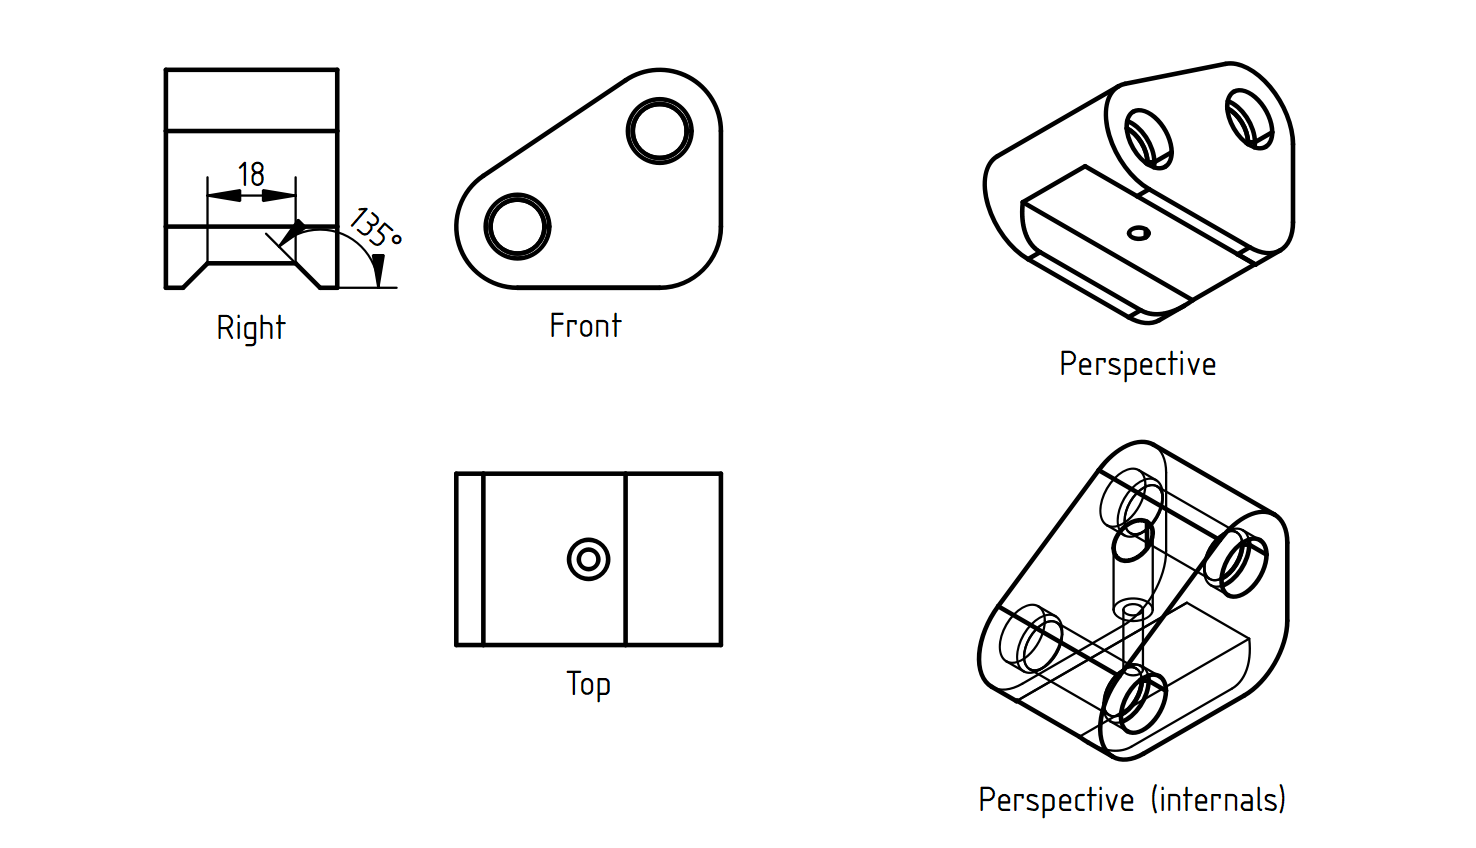
\includegraphics[width=14cm]{figs/vistas_extremo.png}
  \end{center}
  \caption{Vistas del elemento terminal}
  \label{fig:vistas_extremo}
\end{figure}\ 

\subsection{Herramienta electroimán}
\noindent Para dotar al robot de una utilidad, se ha creado una herramienta que contiene un electroimán. Esta herramienta debe de tener la forma 
de la acanaladura anterior para poder encajar en el robot. Además se ha redondeado las esquinas para que visualmente se adapte mejor a la 
forma del extremo del robot. Para unir el conjunto se ha utilizado el propio orificio roscado del electroimán, como se puede ver en la Figura tal
\begin{figure} [ht!]
  \begin{center}
    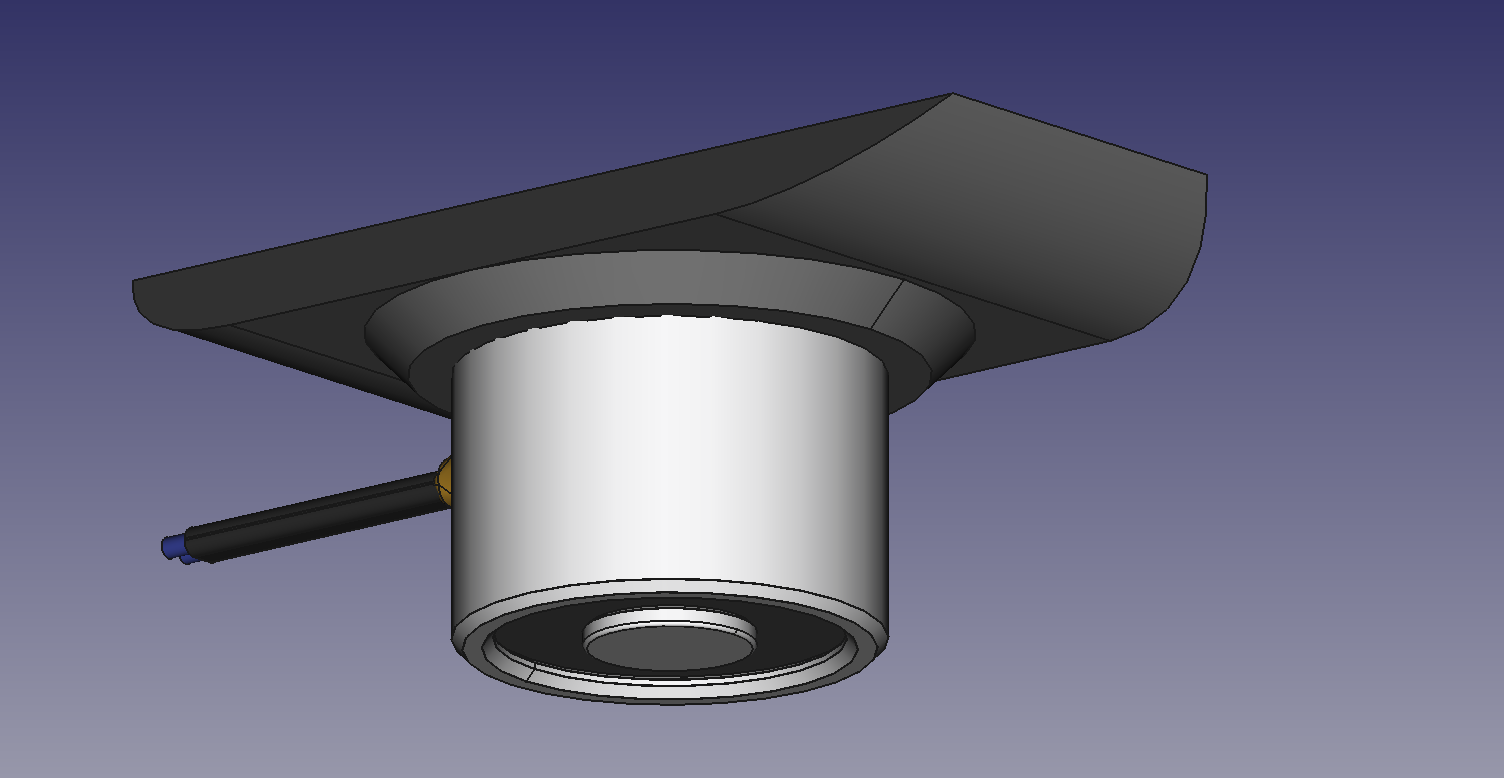
\includegraphics[width=10cm]{figs/electroiman_solo.png}
  \end{center}
  \caption{Herramienta electroimán}
\end{figure}\ 


\subsubsection{Diseño de las poleas dentadas}
Primero, se ha utilizado la herramienta \textit{online} 
gt2-gear-generator\footnote{\url{https://avtehnik.github.io/gt2-gear-genaretor/}} para generar de manera paramétrica el contorno de la polea 
en formato DXF.\\
\begin{figure} [ht!]
  \begin{center}
    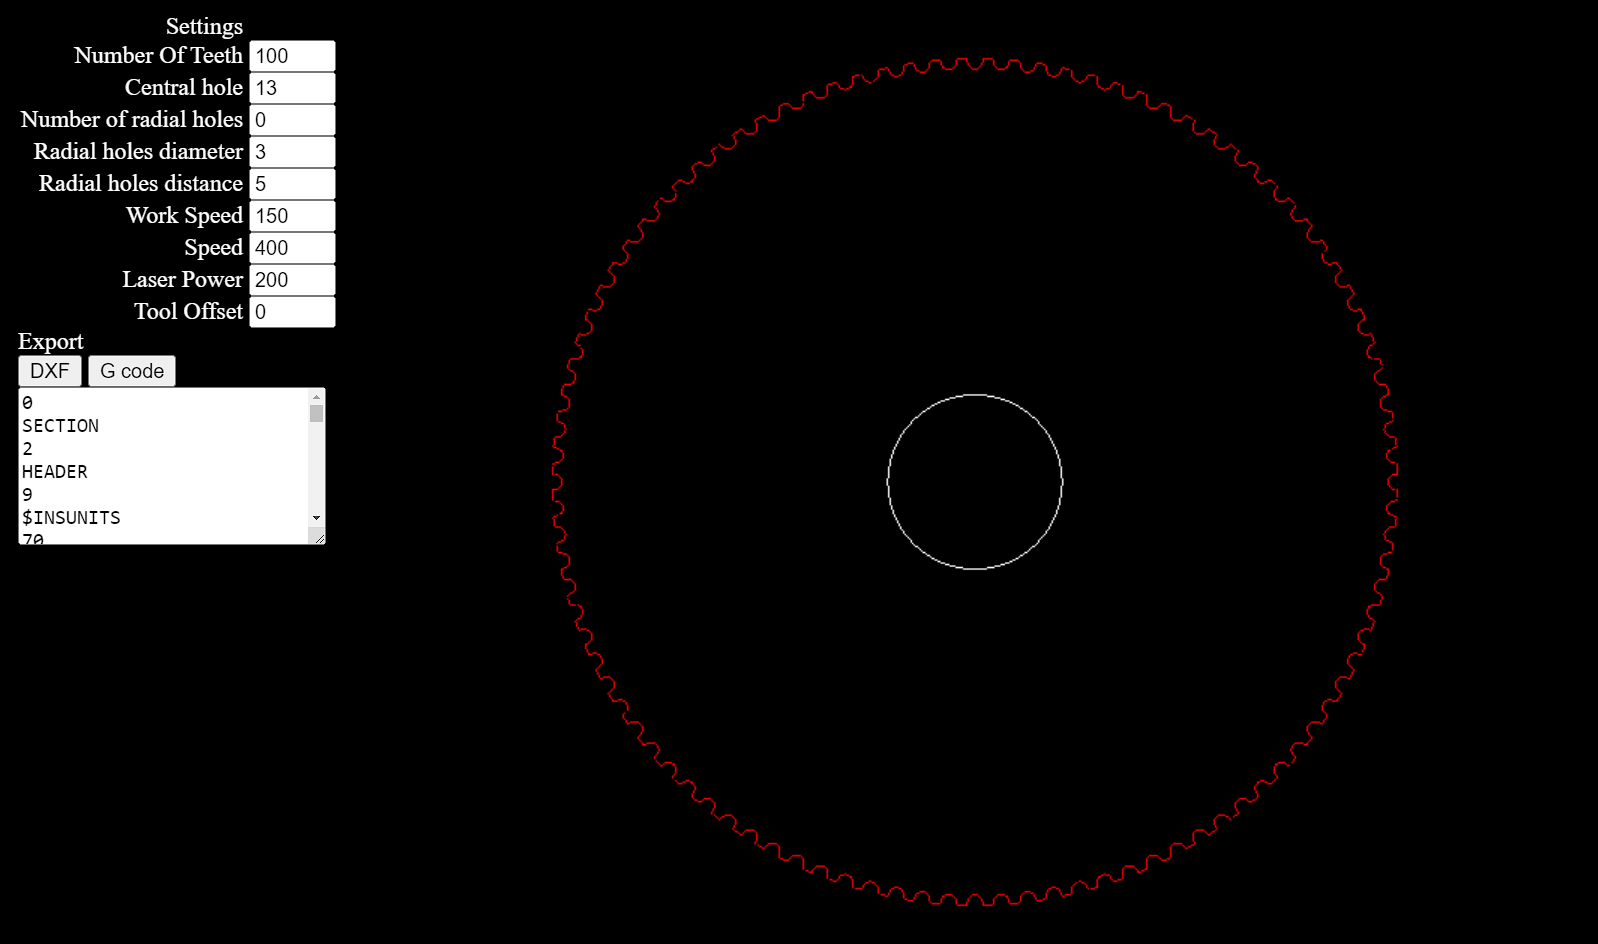
\includegraphics[width=14cm]{figs/dxf_polea.png}
  \end{center}
  \caption{Contorno de la polea de 100 dientes}
\end{figure}\ 
Posteriormente, abrimos el fichero DXF mediante el \textit{workbench} Draft de FreeCad y seleccionamos todos los contornos. A continuación, 
pulsamos en el icono de "Borrador a Croquis" de la barra superior de herramientas y se nos generará un boceto de FreeCad que podremos extruir 
con el \textit{workbench} Part Design. 
\begin{figure} [ht!]
  \begin{center}
    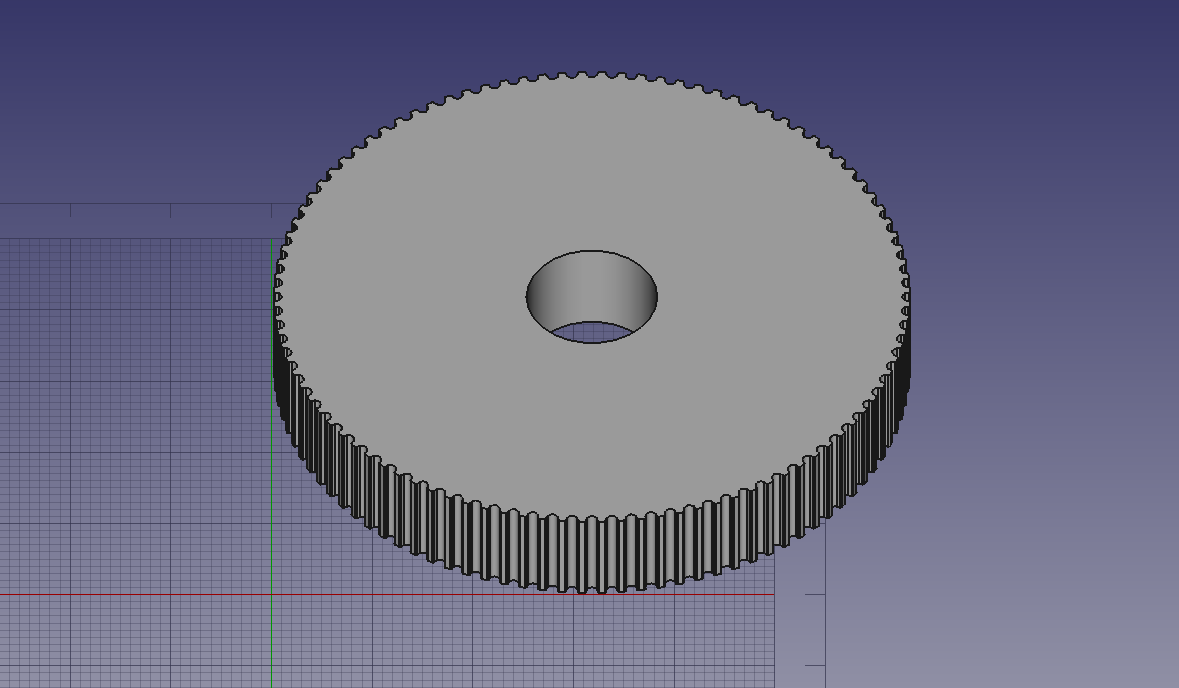
\includegraphics[width=14cm]{figs/polea_freecad.png}
  \end{center}
  \caption{Contorno de la polea de extruido}
\end{figure}\ 

\subsubsection{Mecanismo de tensado de la correa}

\newpage
\section{Impresión y montaje}
En esta sección se exponen todos los detalles a tener en cuenta a la hora de querer replicar este proyecto. Para la impresión 
de G-Arm se ha utilizado una impresora Ender-3 Pro\footnote{\url{https://www.creality.com/products/ender-3-pro-3d-printer}} y un rollo 
de 1Kg de filamento PLA Rojo convencional.
\begin{figure} [h!]
\begin{center}
  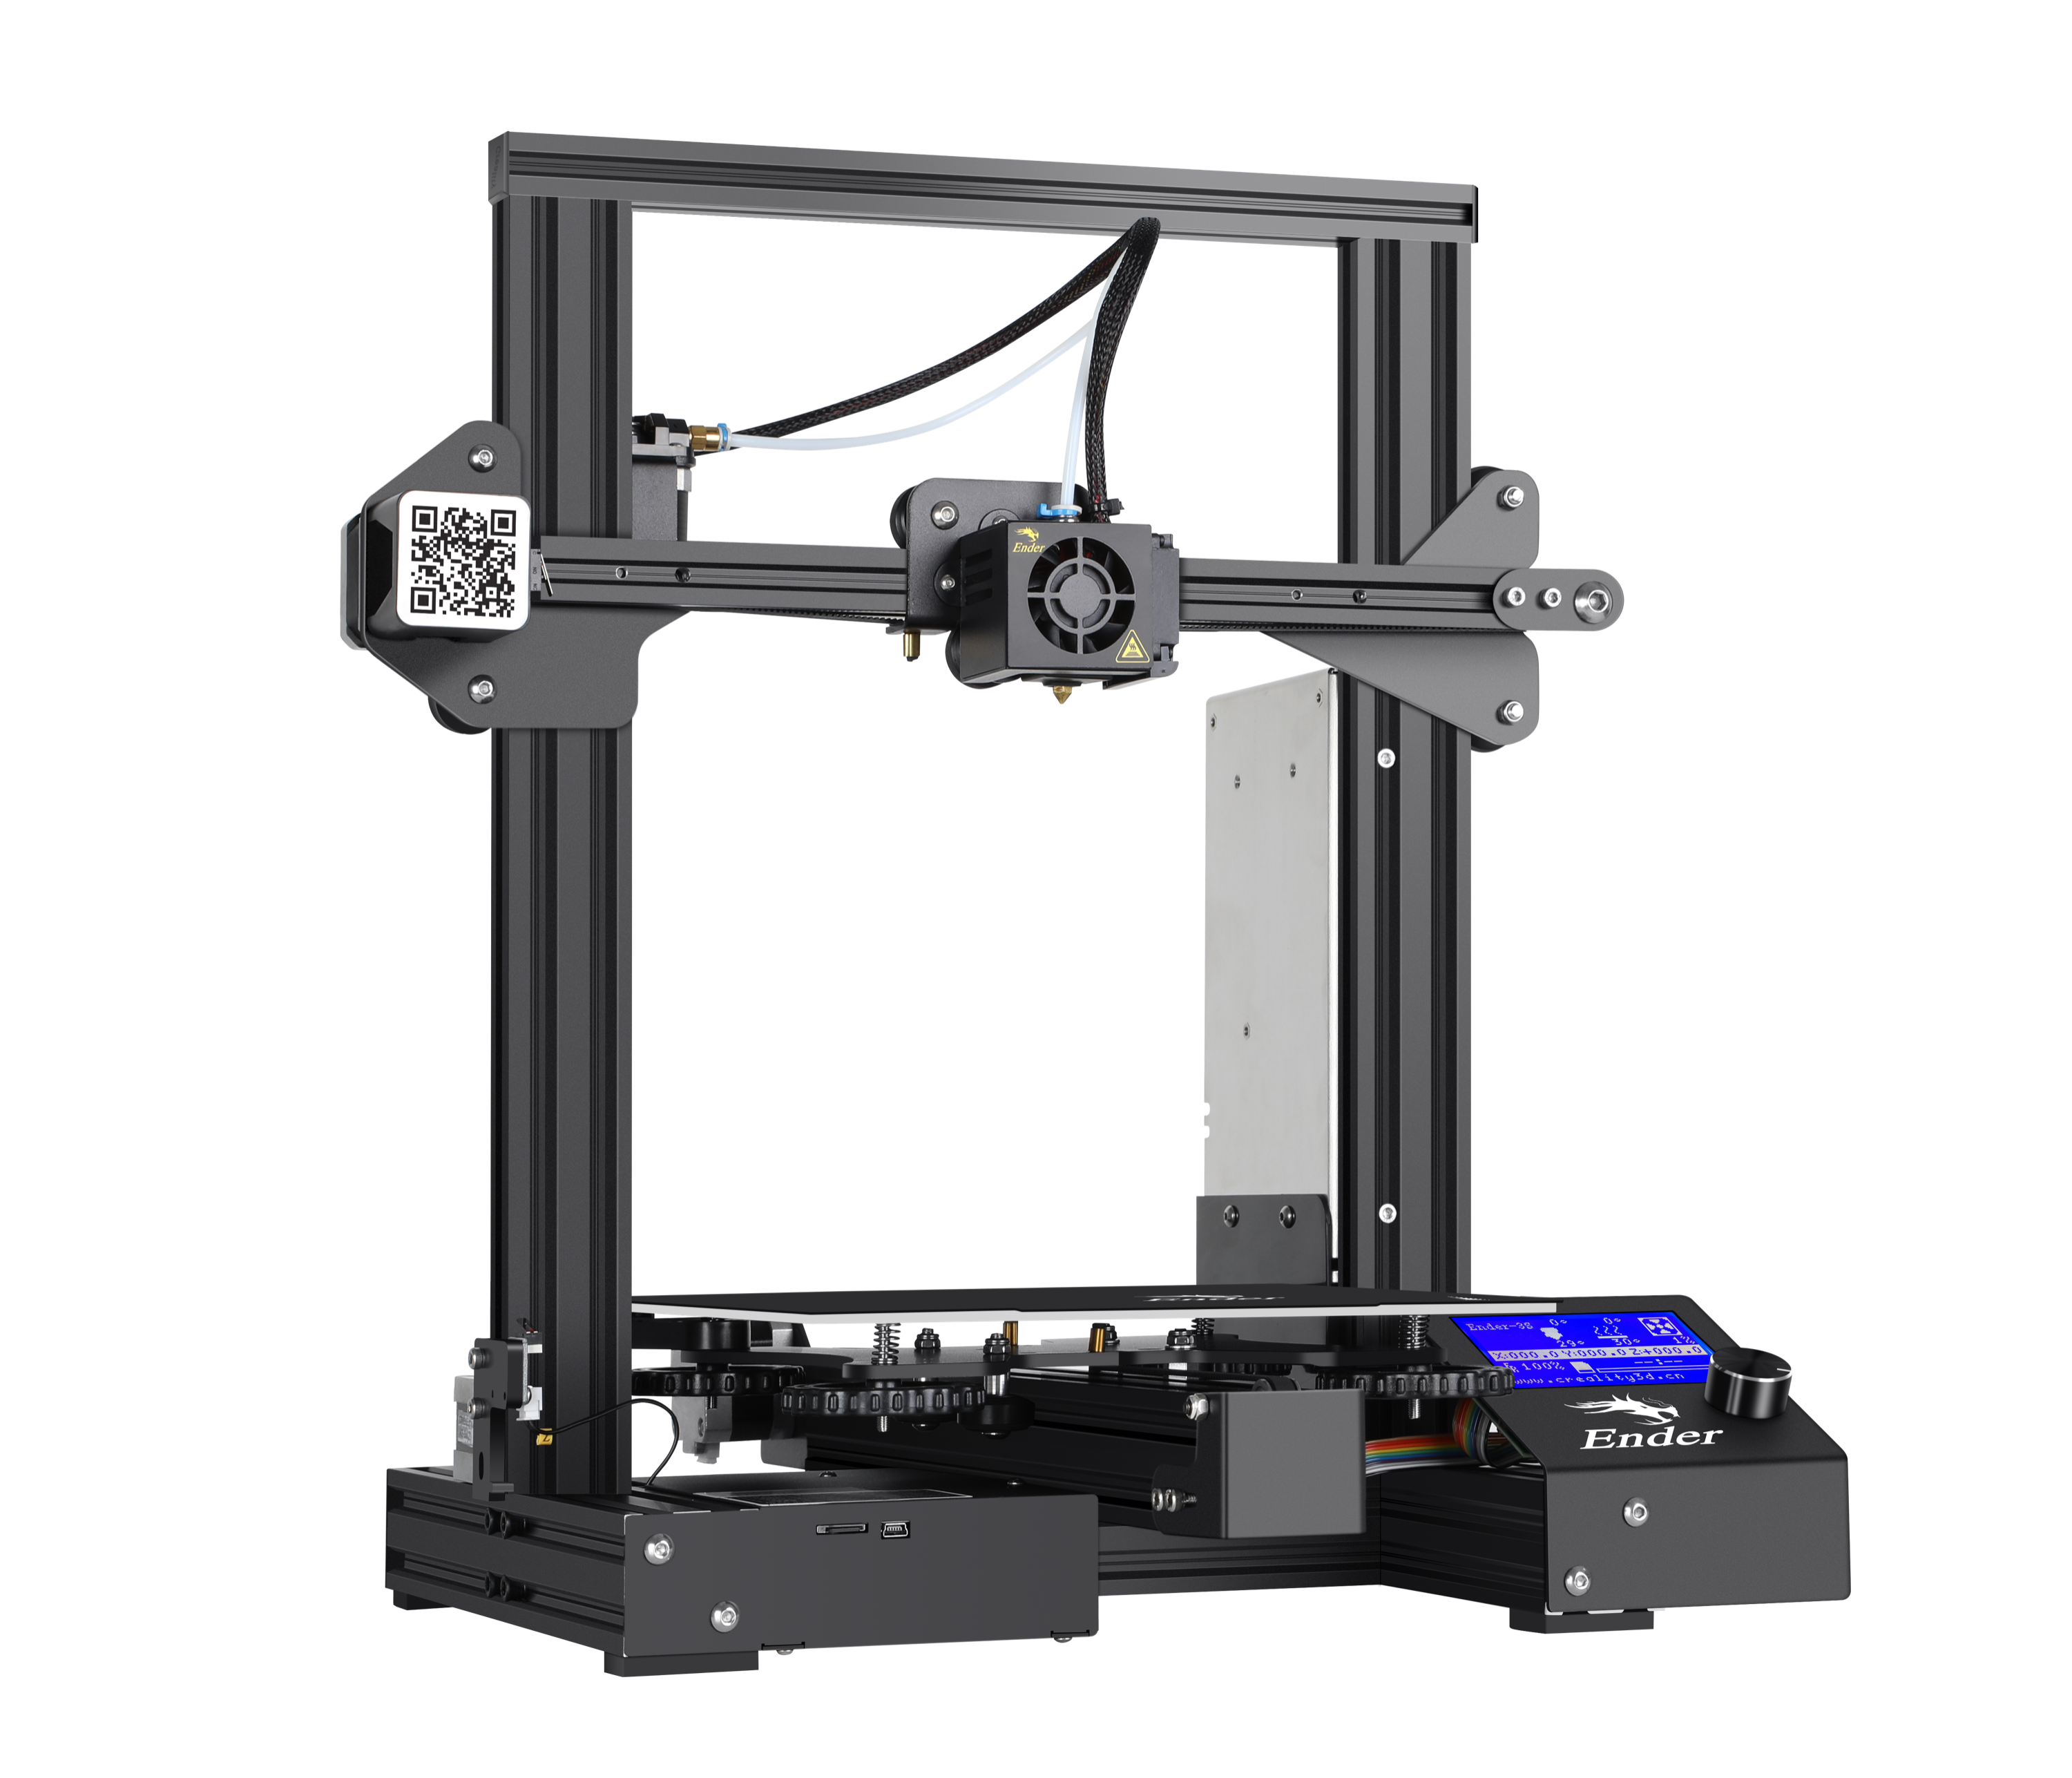
\includegraphics[width=8cm]{figs/ender3.png}
\end{center}
\caption{Ender-3 Pro V1 2017}
\label{fig:ender3pro}
\end{figure}\   

\begin{table}[H]
\begin{center}
\begin{tabular}{|c|c|c|c|}
\hline
\textbf{Componente} & \textbf{Modelo} & \textbf{Cantidad} & \textbf{Precio total} \\
\hline
Motor Nema 17 & 17HS24-2104S & 3 & 56\euro \\
Controlador & TMC2209 & 3 & 10\euro \\
Placa base & MKS DLC32 & 1 & 16\euro \\
Final de carrera & MakerBot (rojo) & 3 & 5\euro \\
Fuente de alimentación & 24V 5A (opcional)\ref{subsec:fuente_alimentacion} & 1 & 15\euro \\
Rodamiento &  F695-2RS Fushi & 22 & 15\euro \\
Rodamiento & F623RS Fushi & 6 & 5.5\euro \\
Polea GT2 & Correa:6mm ID:5mm & 3 & 1.5\euro \\
Correa GT2 & Correa:6mm Largo:252mm & 2 & 3.5\euro \\ 
Correa GT2 &  Correa:6mm Largo:280mm & 1 & 1.8\euro \\ 
Ventilador & 24V 4010 & 1 & 2\euro \\
Electroimán & D20H15mm 3KG 24V & 1 & 3\euro \\
Plástico para imprimir & PLA/PETG 1Kg & 1 & 22\euro \\
\hline
\end{tabular}
\caption{Componentes hardware necesarios}
\label{cuadro:componentes}
\end{center}
\end{table}

\begin{table}[H]
\begin{center}
\begin{tabular}{|c|c|c|}
\hline
\textbf{Componente} & \textbf{Cantidad} & \textbf{Precio total} \\
\hline
Tornillo M3 Allen & 3 & 56\euro \\

\hline
\end{tabular}
\caption{Tornillería necesaria}
\label{cuadro:tornilleria}
\end{center}
\end{table}

El precio total de los componentes necesarios es: 156.3\euro
\begin{table}[H]
\begin{center}
\begin{tabular}{|c|c|c|}
\hline
\textbf{Identificador} & \textbf{Cantidad} & \textbf{Relleno óptimo} \\
\hline
\#1 & 1 & 15\% \\
\hline
\end{tabular}
\caption{Piezas necesarias}
\label{cuadro:piezas}
\end{center}
\end{table}

